\documentclass[11pt,UTF8]{ctexart}
\title{两种流体模型在库埃特与泊肃叶流下的数值模拟情况}
\author{马坤}
\date{2020.1.7}
\usepackage{amsmath}
\usepackage{graphicx}
\usepackage{caption}
\usepackage{hyperref}
\usepackage{subcaption}
\usepackage[left=1in, right=1in, top=1in, bottom=1in]{geometry}
\begin{document}
    \maketitle
    \section{参数选取}
    \par{没有采用无量纲化,部分参数的选取为:
    $$
    H = L = 1m,\rho = 1 kg/m^3,u = 0.01m/s,
    \triangle x=1/199  m,\triangle t = 0.1/199s
    $$
    我们的示性函数为$\phi$,则流体粘性变化函数为:
    $$
    \eta = \eta_s\phi+(1-\phi)\eta_l
    $$
    若我们取$\eta_l=0.02m^2/s$,$rate=\frac{\eta_s}{\eta_l}=50$那么
    $$\eta=(49\phi+1)\eta_l\in[0.02,1]=\nu$$
    由此计算得到
    $$Re = \frac{Hu}{\nu}\in [0.01,0.5]$$}
    \section{平行区域}
    \par{平行区域流体指的是管道中第一层为粘性较大的流体,第二层为粘性较小的流体,
    第三层为粘性较大的流体,如图\ref {img1},其中区域1和区域三粘性一样。}
    \par{假设我们模拟的区域高度为$H=1$(同样假设模拟区域长度
    $L=1$),那么有刻画流体
    区域的示性函数$\phi$:}
    $$
    \phi=
    \begin{cases}
        0.5[-\tanh{\frac{y-1/3}{W}}+1],\text{$y\leq H/2$}\\
        0.5[\tanh{\frac{y-2/3}{W}}+1],\text{$y>H/2$}
    \end{cases}
    $$
    \par{$\phi$理应($W$较小)粘性较大流体里面
    ($y < H/3$ 或者 $y > 2H/3$)为1,理应($W$较小)在粘性较小流体里面$(H/3 < r < 2H/3)$为0。}
    \par{模拟中我们假设粘性比$\frac{\eta_s}{\eta_l}=rate$,其中$\eta_s$为较大的粘性,无维
    度化后的粘性系数$\eta$有如下表达式:
    $$\eta = 1+rate*\phi-\phi.\eqno(1) \label{eqn1}$$
    上述两个表达式上面两个表达式中的$W,rate$都是待定的参数,接下来会通过实验
    选取较好的值。实验中假设的流体的密度均为$\rho=1$,所以有$\eta=\nu$。}
    \subsection{库埃特流}
    \par{在这一节中我们将考察库埃特流,即上面板具有速度,假设为$u_{up}=0.01$,下
    面板速度为$u_{bottom}=0$。流体流动的过程中我们不考虑外力。第一小节是改变$W$,
    第二小节为改变$rate$。}
    \subsubsection{改变$W$}
    \par{如果只考虑单一流体,那么流体的流速应该为线性增长的,但是本文考虑的为大小
    大流体模型,所以流速图会有所差异。此小节的实验,选用的$rate=50$结果图\ref {img2}。}
    \par{观察图\ref {img2}可见,当$W$较大时流速趋于一条直线,尤其是$W=0.5$。这是因为当
    $W$过大时,示性函数$\phi$已经不能较好的反应流体的性质了,这导致了流体粘性比
    小于希望的值;而当$W$较小时示性函数$\phi$较好的反应了流体的性质。观察$W=0.001$
    图像,靠近下面板的大粘性流体速度几乎为0,而靠近上面板的流速为近似为0.01,
    可以理解为粘性大的流体和面板粘在一起。}
    \subsubsection{改变$rate$}
    \par{此小节我们选取的$W=0.01$,然后考察流体稳定后的流速与$rate$之间的关系。
    此时,虽然改变了$rate$的值。可以看见当流体粘性比越小时,流速越趋于一条直线,这和我们的
    理解是相同的。当$rate=1$时,无维度$\eta$就是一个常数,与位置无关,此时画
    出来图片理应为一条直线,与库埃特流精确解一致。但是由于解收敛太慢了,达到此
    过程之前就最大时间停机了。结果见图\ref {img3}。}
    \subsection{泊肃叶流}
    \par{在这一节中我们将考察泊肃叶流,即上下面板没有速度,$u_{up}=u_{bottom}=0$。
    流体流动的过程中我们考虑外力,其中我们外力的选取为$F=\frac{8\rho u_{peak} \eta_s}{H^2}$,其中$u_{peak}=0.1$。如果是单一成分流体,
    并且流体的粘性为$\eta_s$,那么流速应该是一个抛物线,并且峰值为0.1。同样的,
    第一小节是改变$W$,第二小节为改变$rate$。}
    \subsubsection{改变$W$}
    \par{同库埃特流一样,当$W$较大时流速趋于一条抛物线,尤其是$W=0.5$,但是峰值
    不是0.1。这是因为当$W$过大时,示性函数$\phi$已经不能较好的反应流体的性质了,
    这导致了流体粘性比小于希望的值,图像进而类似抛物线,而峰值不为0.1的原因为我们
    外力相对于粘性小的流体来说太大了;而当$W$较小时示性函数$\phi$较好的反应了流体
    的性质。随着$W$的减小,大粘性流体的速度趋于精确解,但小粘性的流体的流速却不停
    的增大,也许会稳定下来。结果见图\ref {img4}。}
    \subsubsection{改变$rate$}
    \par{此图的参数选取与库埃特流的第二小节一样,$Re=500,W=0.1$,不过我们这里改变
    了$rate$,所以进而力也会改变。这个图像就不那么好理解了,尤其是$rate=100$时,
    流体流速很反常,但是当$rate=1$时流体速度和抛物线还是很接近的,这和预期也是很相符。
    但还是当我们取$W=0.01,W=0.5$时,情况有所变化。结果分别为图\ref {img5}、图\ref {img6}、图\ref {img7}。图\ref {img27}为了查看$rate=100$,在不同的$W$的情况下是否还是会出现反常的情况}
    \section{圆形区域}
    \par{在流体中的圆形固体指的是在正方形流体区域有一个
    圆心在中心的固体,我们在此模拟中可以将其看成一个粘性
    较大的流体。假设正方形区域高为$H=1$,长为$L=1$。
    圆形位于$(1/2,1/2)$,半径长$R=1/4$,如图\ref {img8}。}
    \par{进一步假设刻画流体
    区域的示性函数,
    $$\phi=0.5[-\tanh \frac{2.4(r-1/4)}{W} + 1],r=\sqrt{(x-1/2)^2+(y-1/2)^2}$$
    $\phi$理应($W$较小)粘性较大流体(圆形区域内$r<R$)里面为1,理应($W$较小)在粘性
    较小流体(圆形区域外$r>R$)里面为0。}
    \par{模拟中我们假设粘性比$\frac{\eta_s}{\eta_l}=rate$,其中
    $\eta_s$为较大的粘性(圆形的区域内的流体),$\eta_l$为较小的
    粘性(圆形的区域外的流体),无维度化后的粘性系数$\eta$有如下表达式:
    $$\eta = 1+rate*\phi-\phi.\eqno(2)$$
    上述两个表达式上面两个表达式中的$W,rate$都是待定的参数,接下来
    会通过实验选取较好的值。实验中假设的流体的密度均为$\rho=1$,所以
    有$\eta=\nu$。}
    \subsection{库埃特流}
    \par{面对库埃特流实验了一个情况,$W=0.1,rate=50$。下图为3维
    的情况与2维的情况。其中2维图中$x=0,x=0.5$意味着截取的平面为长的开始点
    $(0,0)$与中间点$(L/2,0)$,即图7中的坐标系下的坐标。结果见图\ref {img9}、图\ref {img10}。}
    \subsubsection{W变化}
    \par{此时我们考察的是在圆形区域库埃特流情况下,固定$rate=50$,流体速度随着$W$的变化情况。
    由于此时的速度是一个二元函数,所以在这只能给出速度某些截面的速度分布,类似于图\ref {img9}的方法。
    截取的平面分别为$x=0,x=0.25,x=0.5$,具体结果见图\ref {img11}、图\ref {img12}、图\ref {img13}。}
    \subsubsection{rate变化}
    \par{此时我们考察的是在圆形区域库埃特流情况下,固定$W=0.1$,流体速度随着$rate$的变化情况。
    类似2.1.1节的情况,截取的平面分别为$x=0,x=0.25,x=0.5$,具体结果见图\ref {img14}、图\ref {img15}、图\ref {img16}。}
    \subsection{泊肃叶流}
    \par{面对泊肃叶流实验了一个情况,$W=0.1,rate=50$。正如
    之前,此时力是恒定的,所以其选取就有了一定麻烦。当力取得较大$F=\frac{8\rho u_{peak} \eta_s}{H^2}$时,
    数值算法崩溃了,当取得较小时$F=\frac{8\rho u_{peak} \eta_l}{H^2}$,
    稳定结果,但是结果也有一些问题。其中2维图中$x=0,x=0.5$意味着截取的平面为长的开始点
    $(0,0)$与中间点$(L/2,0)$。结果见图\ref {img17}、图\ref {img18}。}
    \subsubsection{W变化}
    \par{此时我们考察的是在圆形区域泊肃叶流情况下,固定$rate=50$,流体速度随着$W$的变化情况。
    由于此时的速度是一个二元函数,所以在这只能给出速度某些截面的速度分布,类似于图9的方法。
    截取的平面分别为$x=0,x=0.25,x=0.5$,具体结果见图\ref {img19}、图\ref {img20}、图\ref {img21}。前面几节的结果是
    当$W$越大得到的解更接近抛物线,可是这里却有所不同——$W$越大曲线越趋于扁平。我认为这是由于
    $F$取值较小导致的结果,至于更深入的解释为什么$F$取较小的值会如此暂时没有有所结果。}
    \subsubsection{rate变化}
    \par{此时我们考察的是在圆形区域泊肃叶流情况下,固定$W=0.1$,流体速度随着$rate$的变化情况。
    类似2.1.1节的情况,截取的平面分别为$x=0,x=0.25,x=0.5$,具体结果见图\ref {img22}、图\ref {img23}、图\ref {img24}。}
    \section{MATLAB模拟}
    \par{此节的目的是利用matlab的bvp4c函数来解决两点边值ode问题,验证LBM是否真的解决了对应的物理问题。
    我们先给出合适的两点边值问题的形式,此处我们只测试了平行区域,因为只有平行区域是ode,圆形区域是pde问题。}
    $$
    \frac{\partial}{\partial y} (\eta \frac{\partial u}{\partial y})=
    \begin{cases}
        0,\text{cutte flow}\\
        F = \frac{8\rho u_{peak} \eta_s}{H^2},\text{Poiseuille flow}
    \end{cases}
    $$
    $$
    u(0) = 0,u(1)=
    \begin{cases}
        0,\text{cutte flow}\\
        u_{peak},\text{Poiseuille flow}
    \end{cases}
    $$
    \par{此处给出了具体的两点边值表达式以及边值条件,注意表达式中$\eta$是一个分段函数,具体的表达式是等式\ref {eqn1}。接下来是利用
    matlab中bvp4c解ode以及对比LBM的计算结果。具体结果参考图\ref {img25},图\ref {img26}。}
    \newpage
%pic1
    \begin{figure}[h]
        \centerline{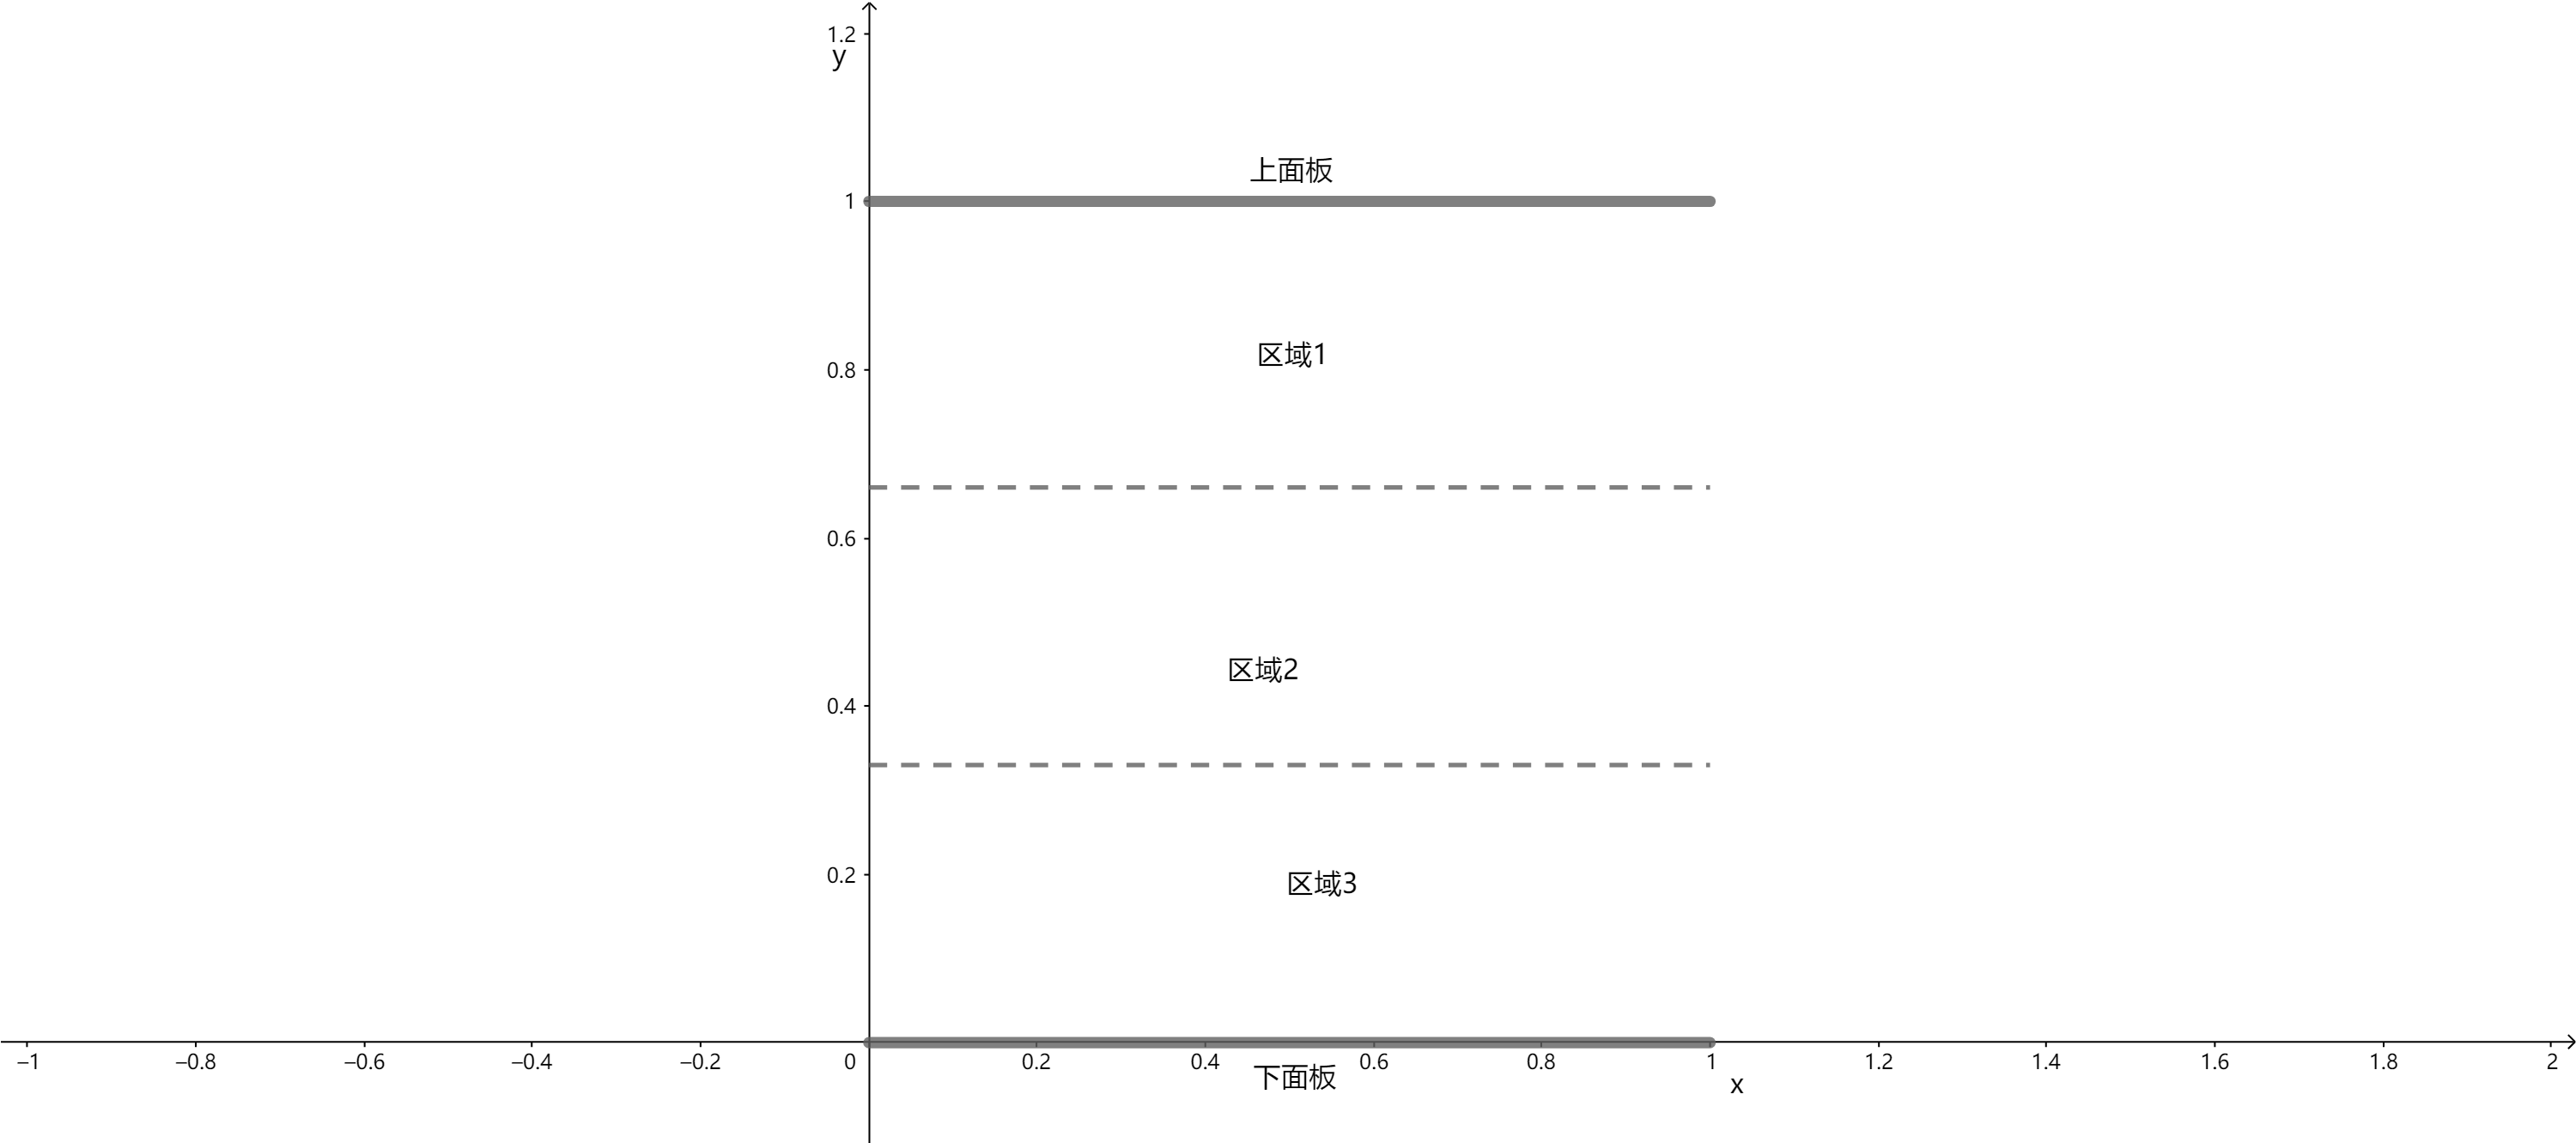
\includegraphics[width=0.8\textwidth]{parallel.png}}
        \caption{平行区域示意图:$x$为水平轴,$y$为垂直轴,由于模拟区域为$H=L=1$,所以数值算法模拟区域为$(x,y)\in [0,1]\times [0,1]$。}
        \label{img1}
    \end{figure}
%pic2
    \begin{figure}[h]
        \centerline{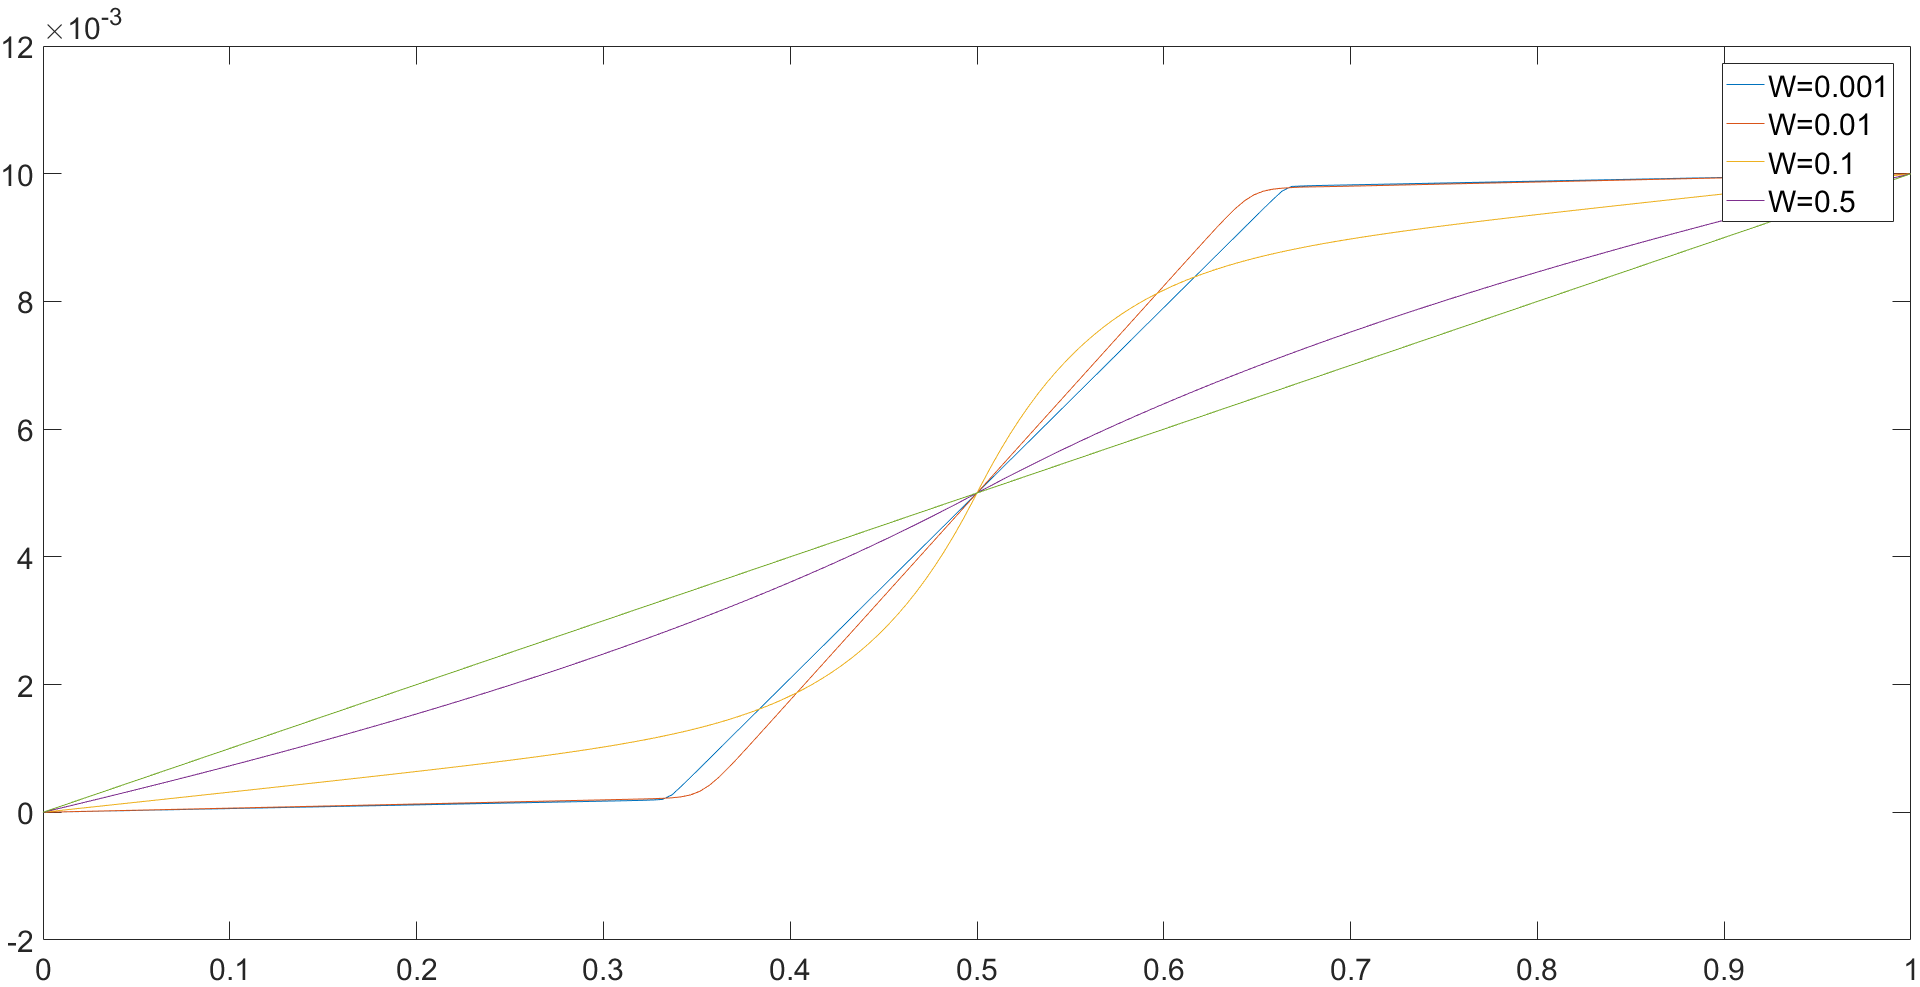
\includegraphics[width=0.8\textwidth]{Parall_C_W/untitled.png}}
        \caption{平行区域下库埃特流随着$W$变化的图像:模拟区域为$(x,y)\in [0,1]\times [0,1]$,其中固定$rate=50$,选取$F=0$。}
        \label{img2}
    \end{figure}
%pic3
    \begin{figure}[h]
        \centerline{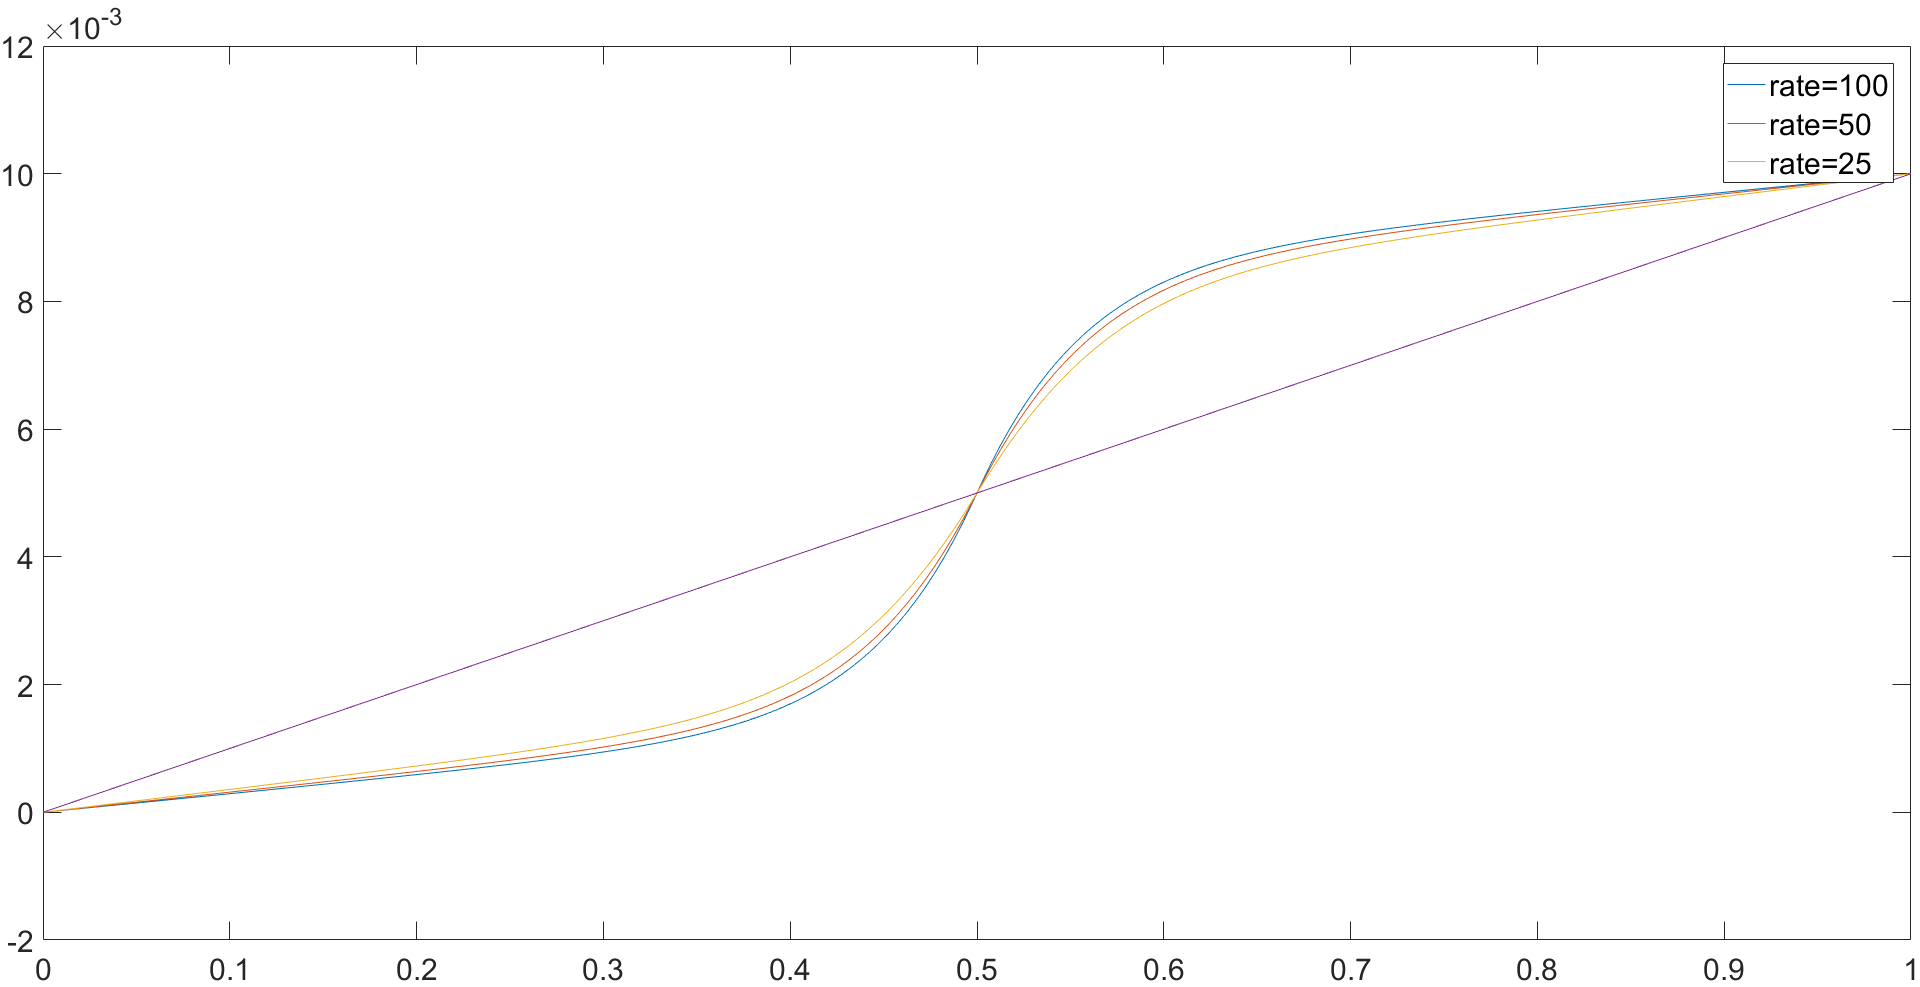
\includegraphics[width=0.8\textwidth]{Parall_C_rate/untitled.png}}
        \caption{平行区域下埃特流随着$rate$变化的图像:模拟区域为$(x,y)\in [0,1]\times [0,1]$,其中固定$W=0.01$,选取$F=0$。}
        \label{img3}
    \end{figure}
%pic4
    \begin{figure}[p]
        \centerline{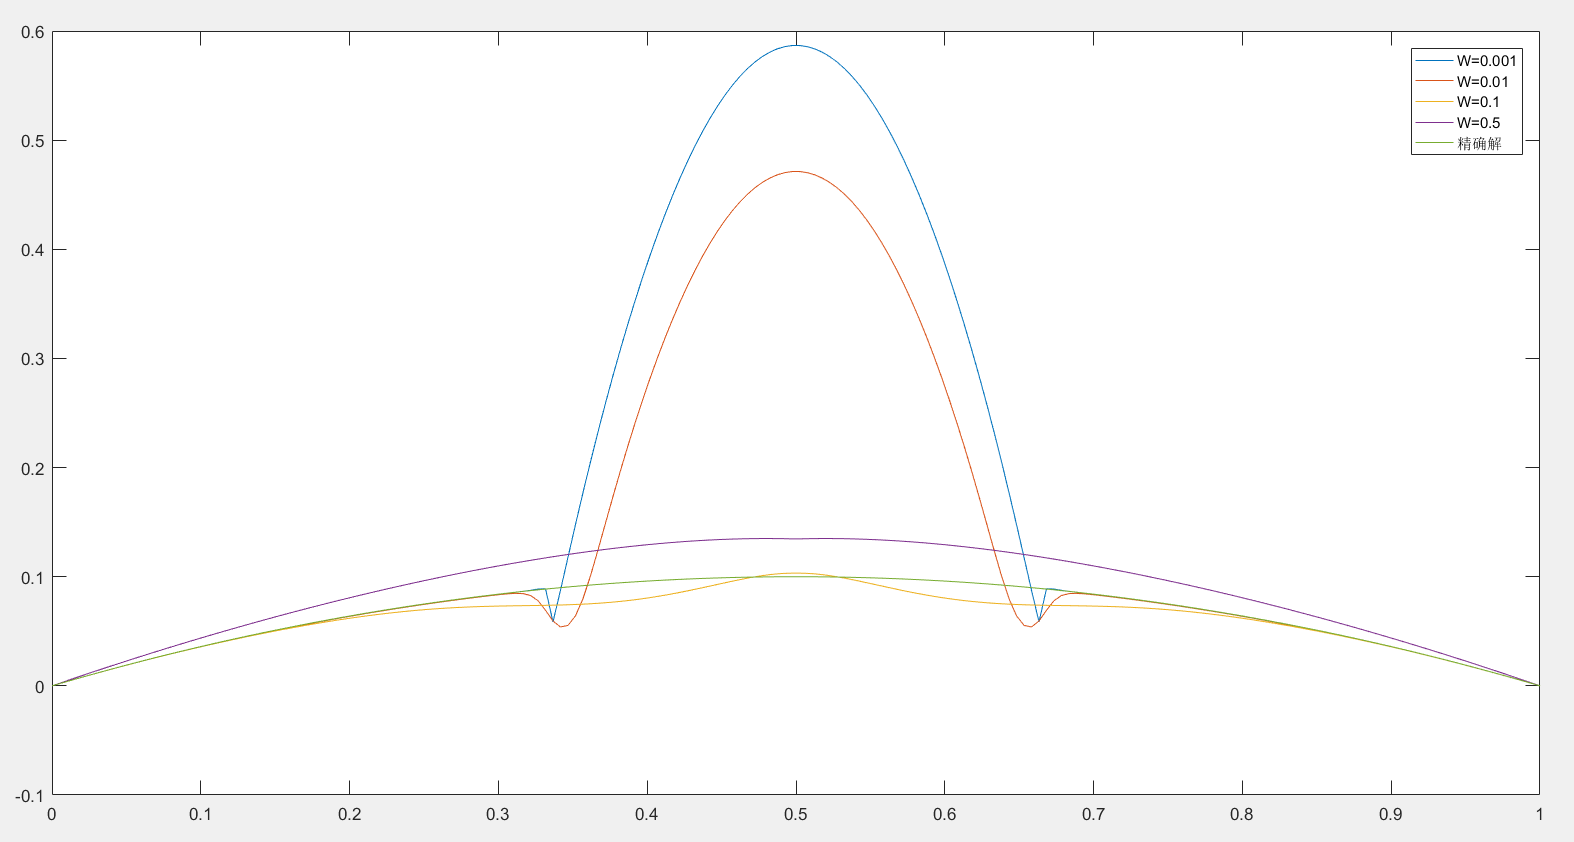
\includegraphics[width=0.8\textwidth]{Poiseuille_W.png}}
        \caption{平行区域下泊肃叶流随着$W$变化的图像:模拟区域为$(x,y)\in [0,1]\times [0,1]$,其中固定$rate=50$,选取$Re=500,F=\frac{8\rho u_{peak} \eta_s}{H^2}$,其中$u_{peak}=0.1$。}
        \label{img4}
    \end{figure}
%pic5
    \begin{figure}[h]
        \centerline{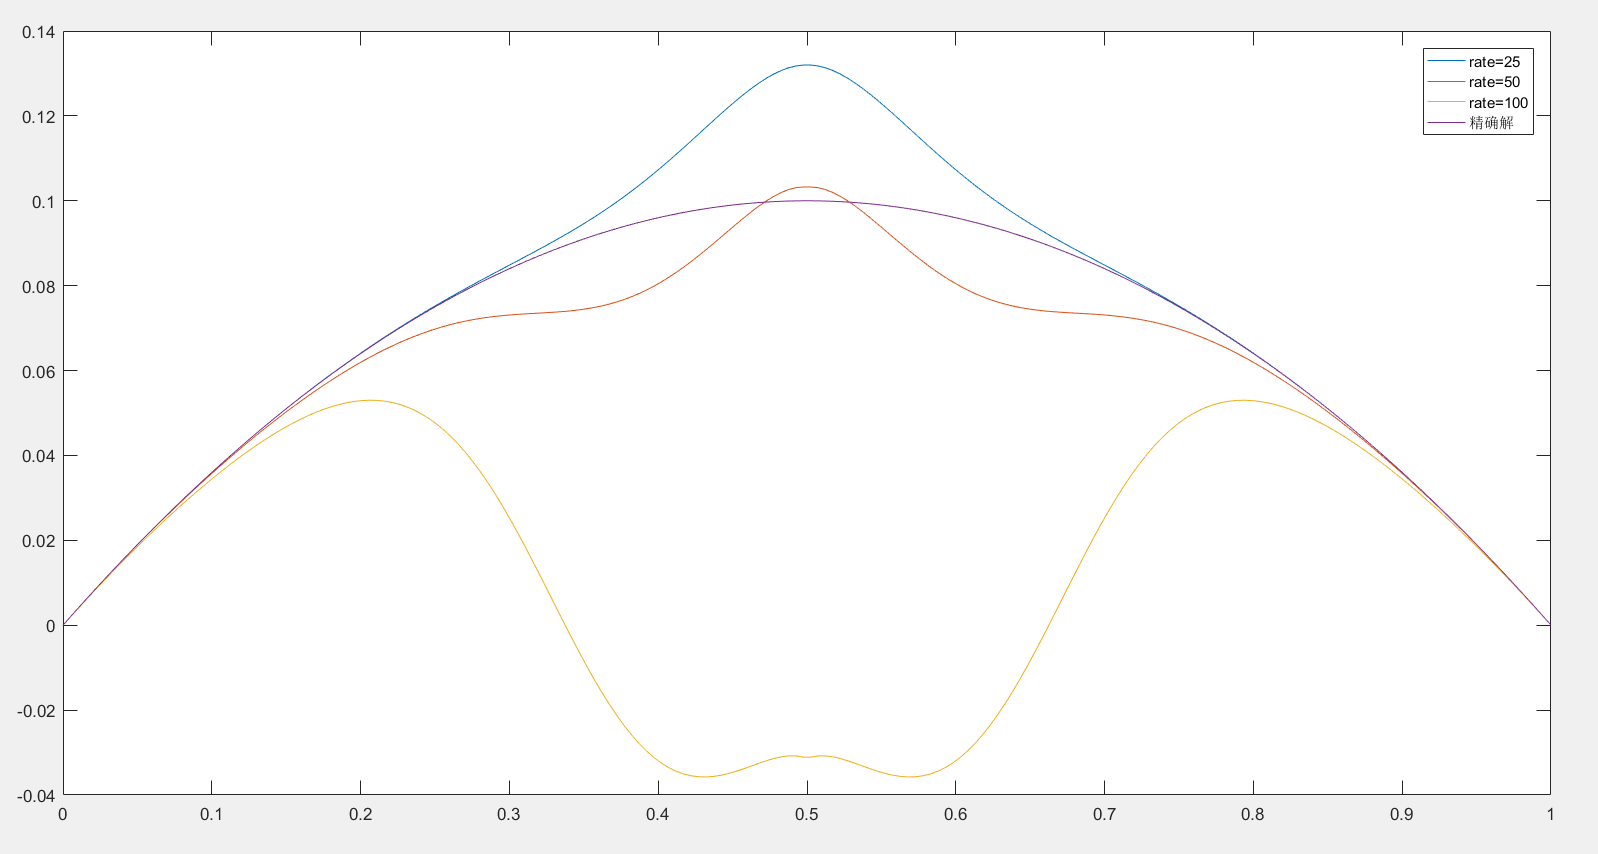
\includegraphics[width=0.8\textwidth]{Poiseuille_rate_W_0_1.png}}
        \caption{平行区域下泊肃叶流随着$rate$变化的图像:模拟区域为$(x,y)\in [0,1]\times [0,1]$,其中固定$W=0.1$,选取$Re=500,F=\frac{8\rho u_{peak} \eta_s}{H^2}$,其中$u_{peak}=0.1$。}
        \label{img5}
    \end{figure}
%pic6
    \begin{figure}[h]
        \centerline{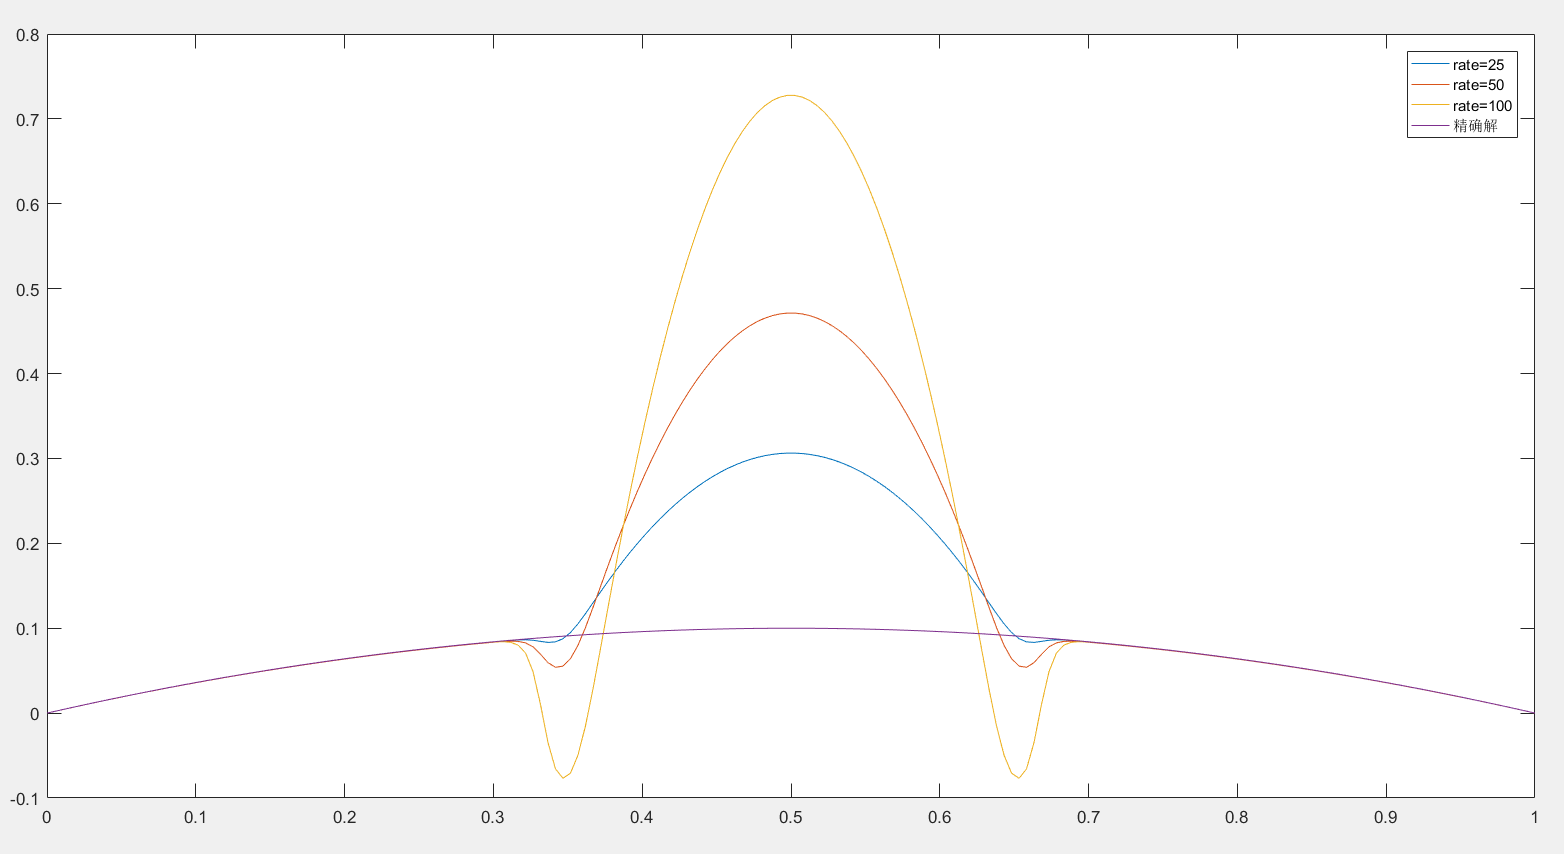
\includegraphics[width=0.8\textwidth]{Poiseuille_rate_W_0_01.png}}
        \caption{平行区域下泊肃叶流随着$rate$变化的图像:模拟区域为$(x,y)\in [0,1]\times [0,1]$,其中固定$W=0.01$,选取$Re=500,F=\frac{8\rho u_{peak} \eta_s}{H^2}$,其中$u_{peak}=0.1$。}
        \label{img6}
    \end{figure}
%pic7
    \begin{figure}[h]
        \centerline{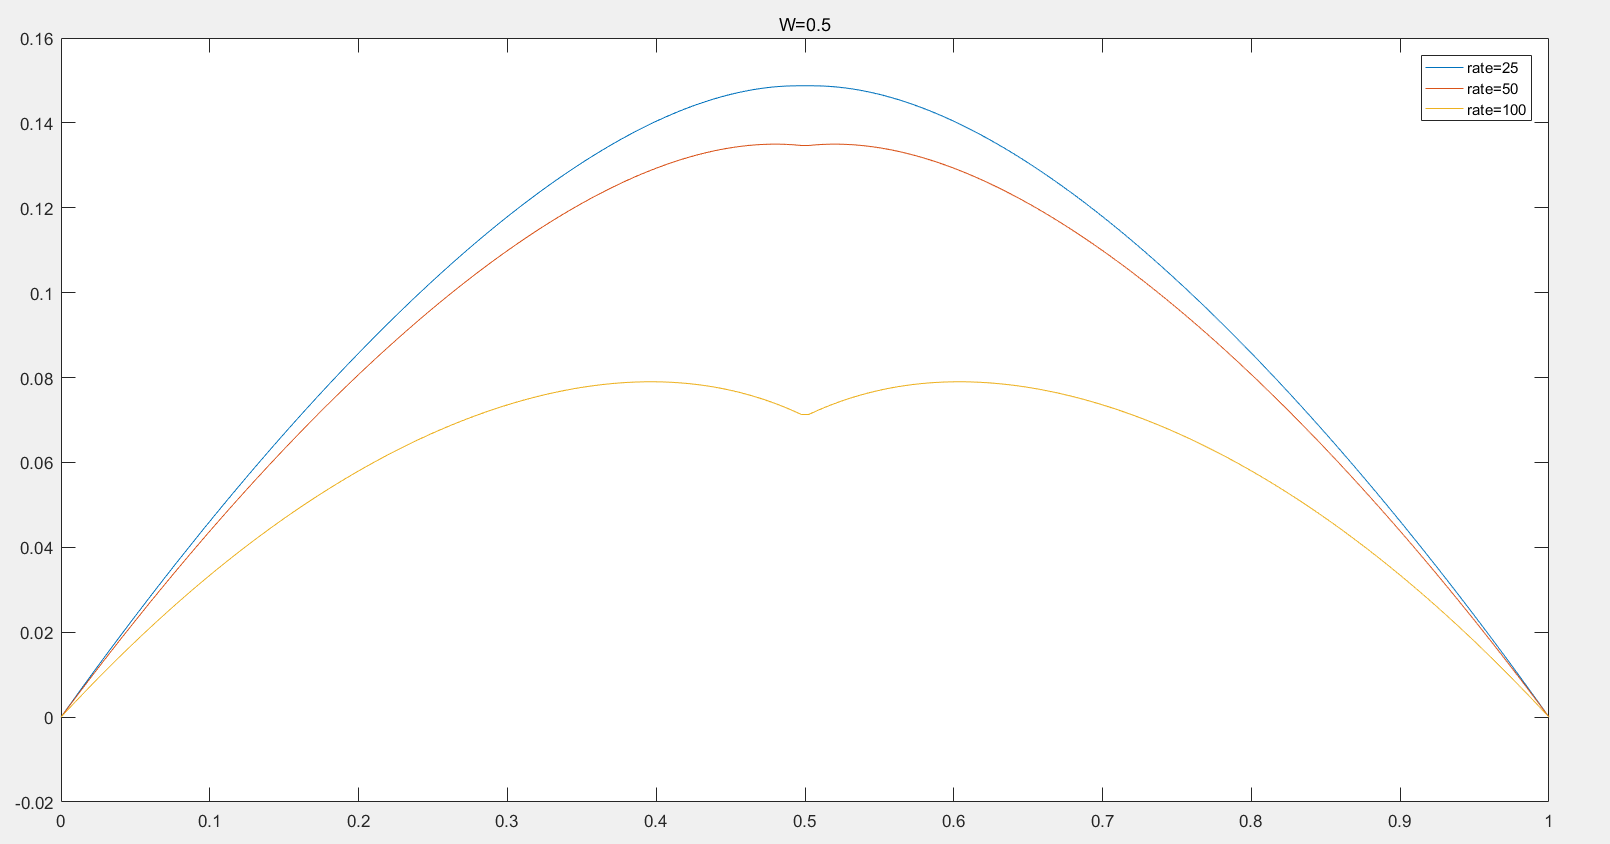
\includegraphics[width=0.8\textwidth]{Poiseuille_rate_W_0_5.png}}
        \caption{平行区域下泊肃叶流随着$rate$变化的图像:模拟区域为$(x,y)\in [0,1]\times [0,1]$,其中固定$W=0.5$,选取$Re=500,F=\frac{8\rho u_{peak} \eta_s}{H^2}$,其中$u_{peak}=0.1$。}
        \label{img7}
    \end{figure}
%pic8
    \begin{figure}[h]
        \centerline{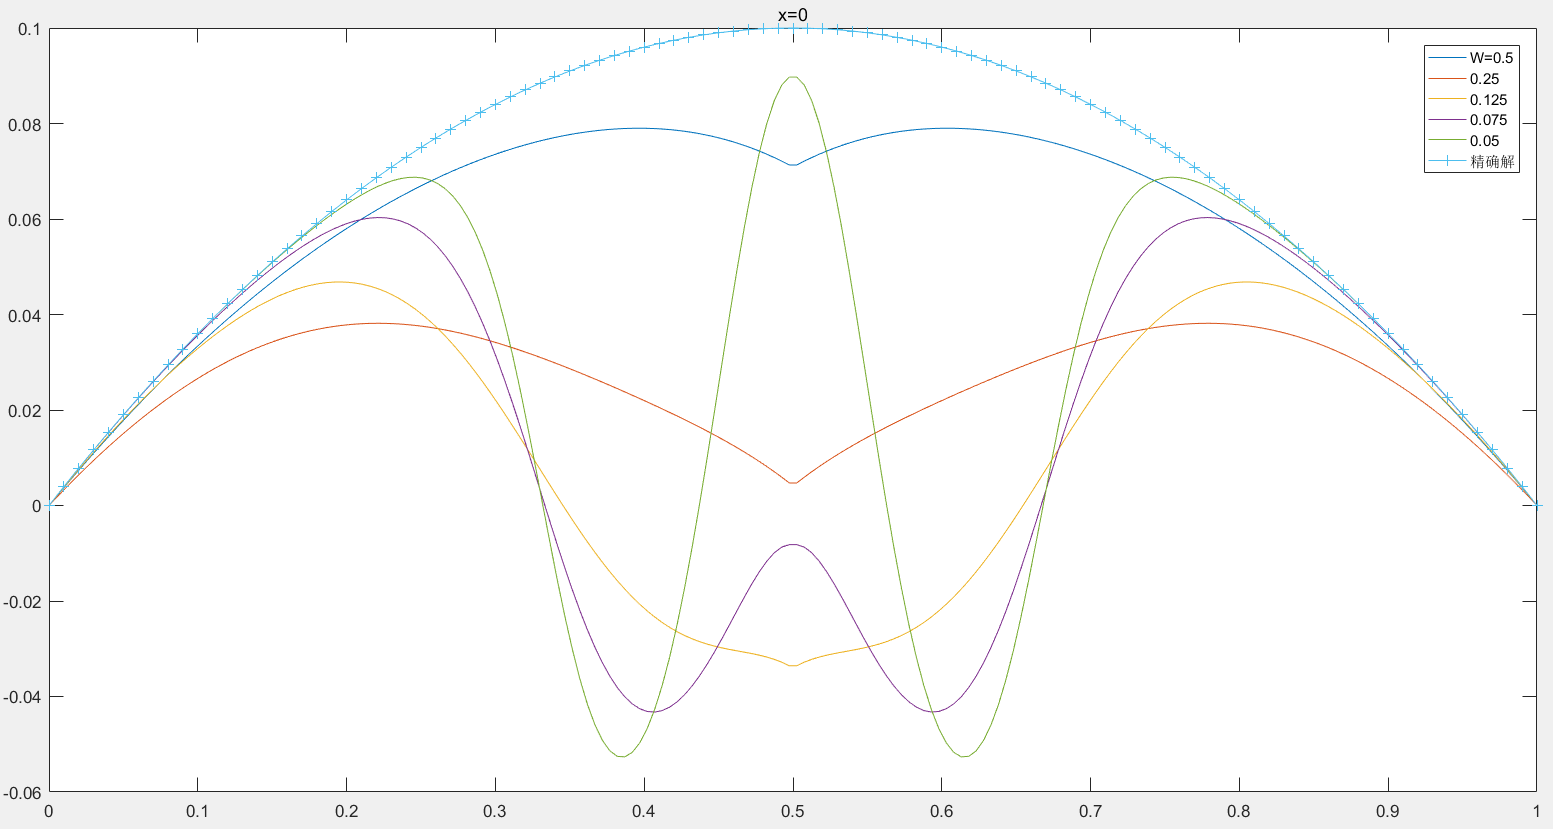
\includegraphics[width=0.8\textwidth]{check_rate_100.PNG}}
        \caption{平行区域下泊肃叶流固定$rate=100$,随着$W$变化的图像:模拟区域为$(x,y)\in [0,1]\times [0,1]$,其中固定$rate=100$,选取$Re=500,F=\frac{8\rho u_{peak} \eta_s}{H^2}$,其中$u_{peak}=0.1$。}
        \label{img27}
    \end{figure}
%pic8
    \begin{figure}[h]
        \centerline{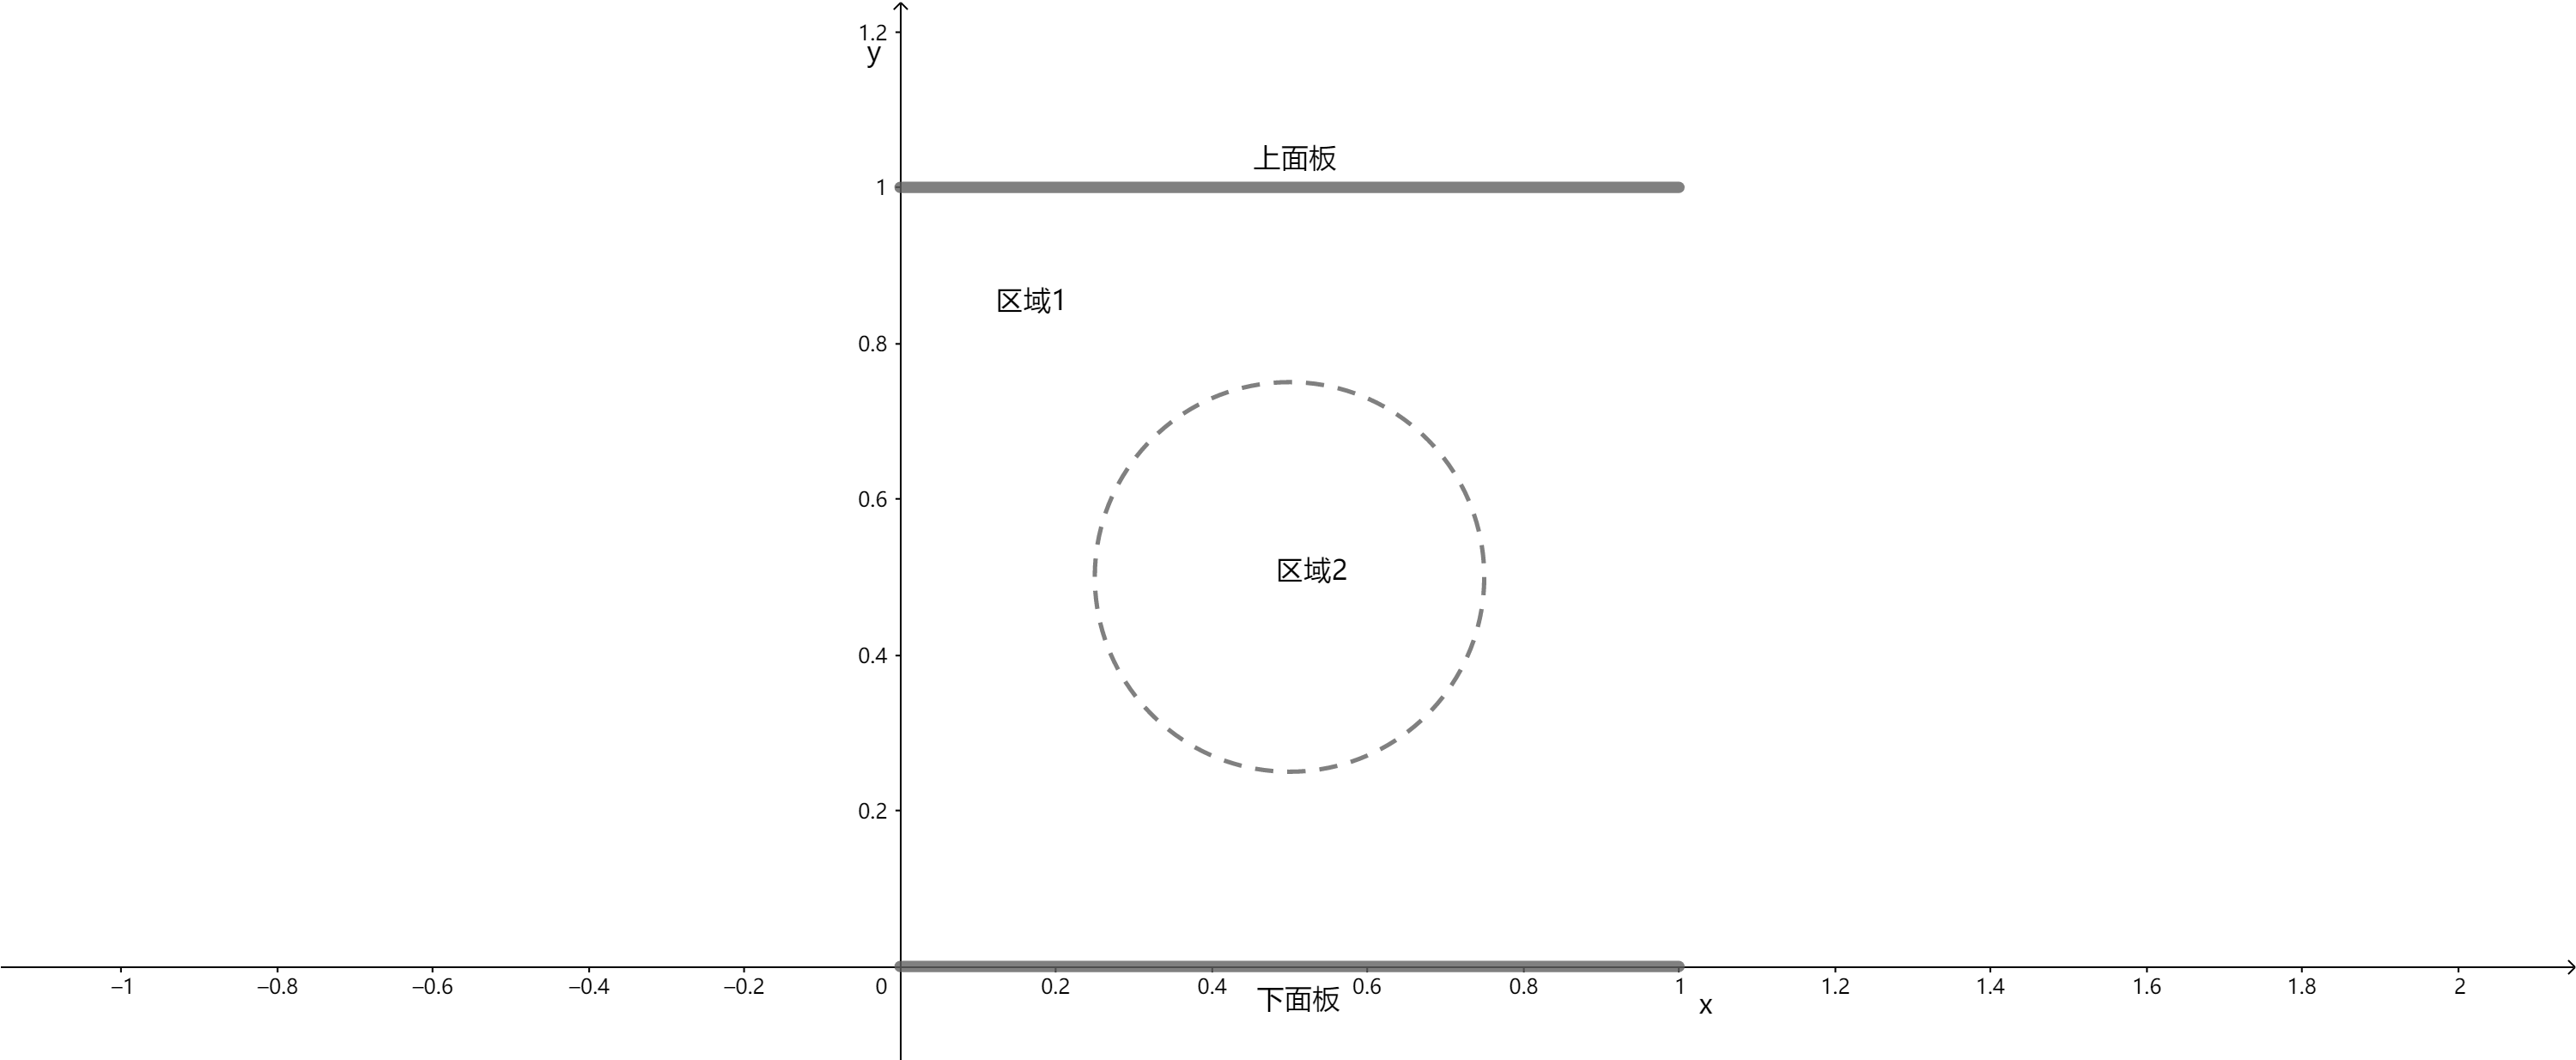
\includegraphics[width=0.8\textwidth]{circle.png}}
        \caption{圆形区域示意图:$x$为水平轴,$y$为垂直轴,由于模拟区域为$H=L=1$,所以数值算法模拟区域为$(x,y)\in [0,1]\times [0,1]$。}
        \label{img8}
    \end{figure}
%pic10
    \begin{figure}[h]
        \centerline{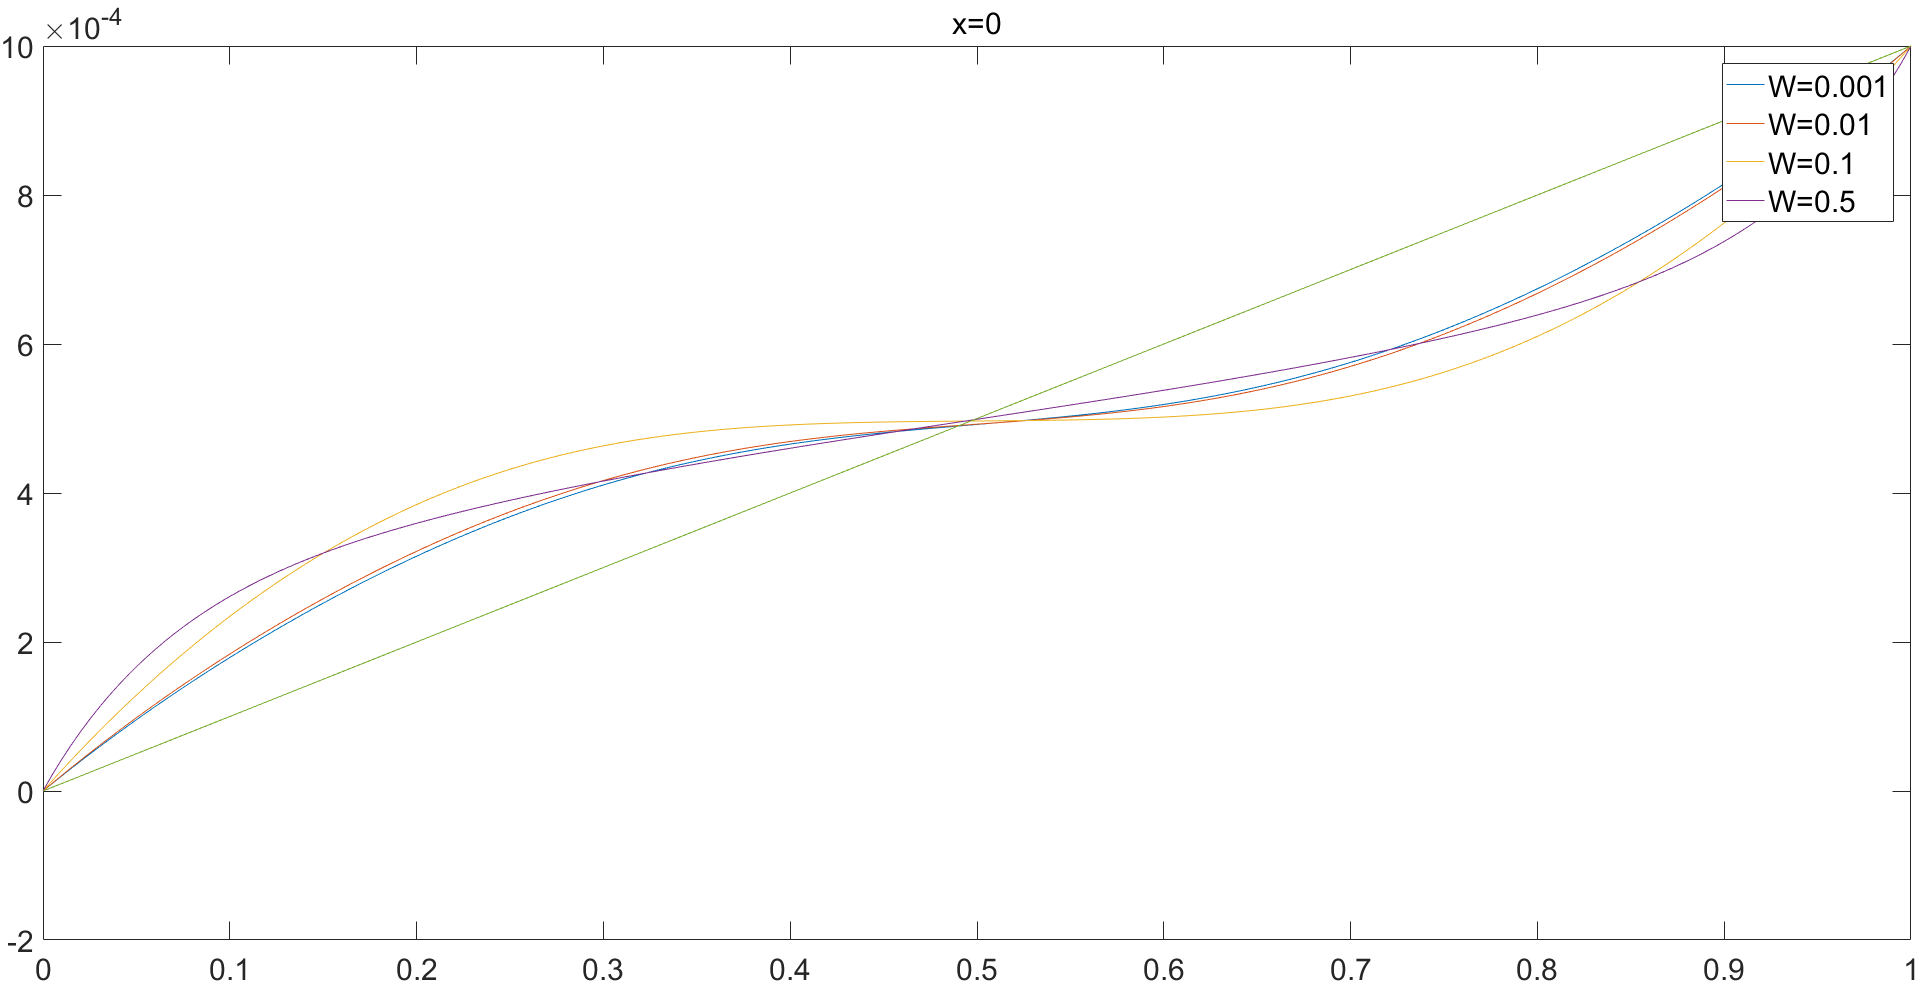
\includegraphics[width=0.8\textwidth]{Circul_P_W/x=0.png}}
        \caption{圆形区域下库埃特流速度随着$W$的变化情况:模拟区域为$(x,y)\in [0,1]\times [0,1]$,其中$rate=50,F=0$,标题中$x=0$表示曲线为在对应$x$轴位置的3维图形的截线。}
        \label{img11}
    \end{figure}
%pic11
    \begin{figure}[h]
        \centerline{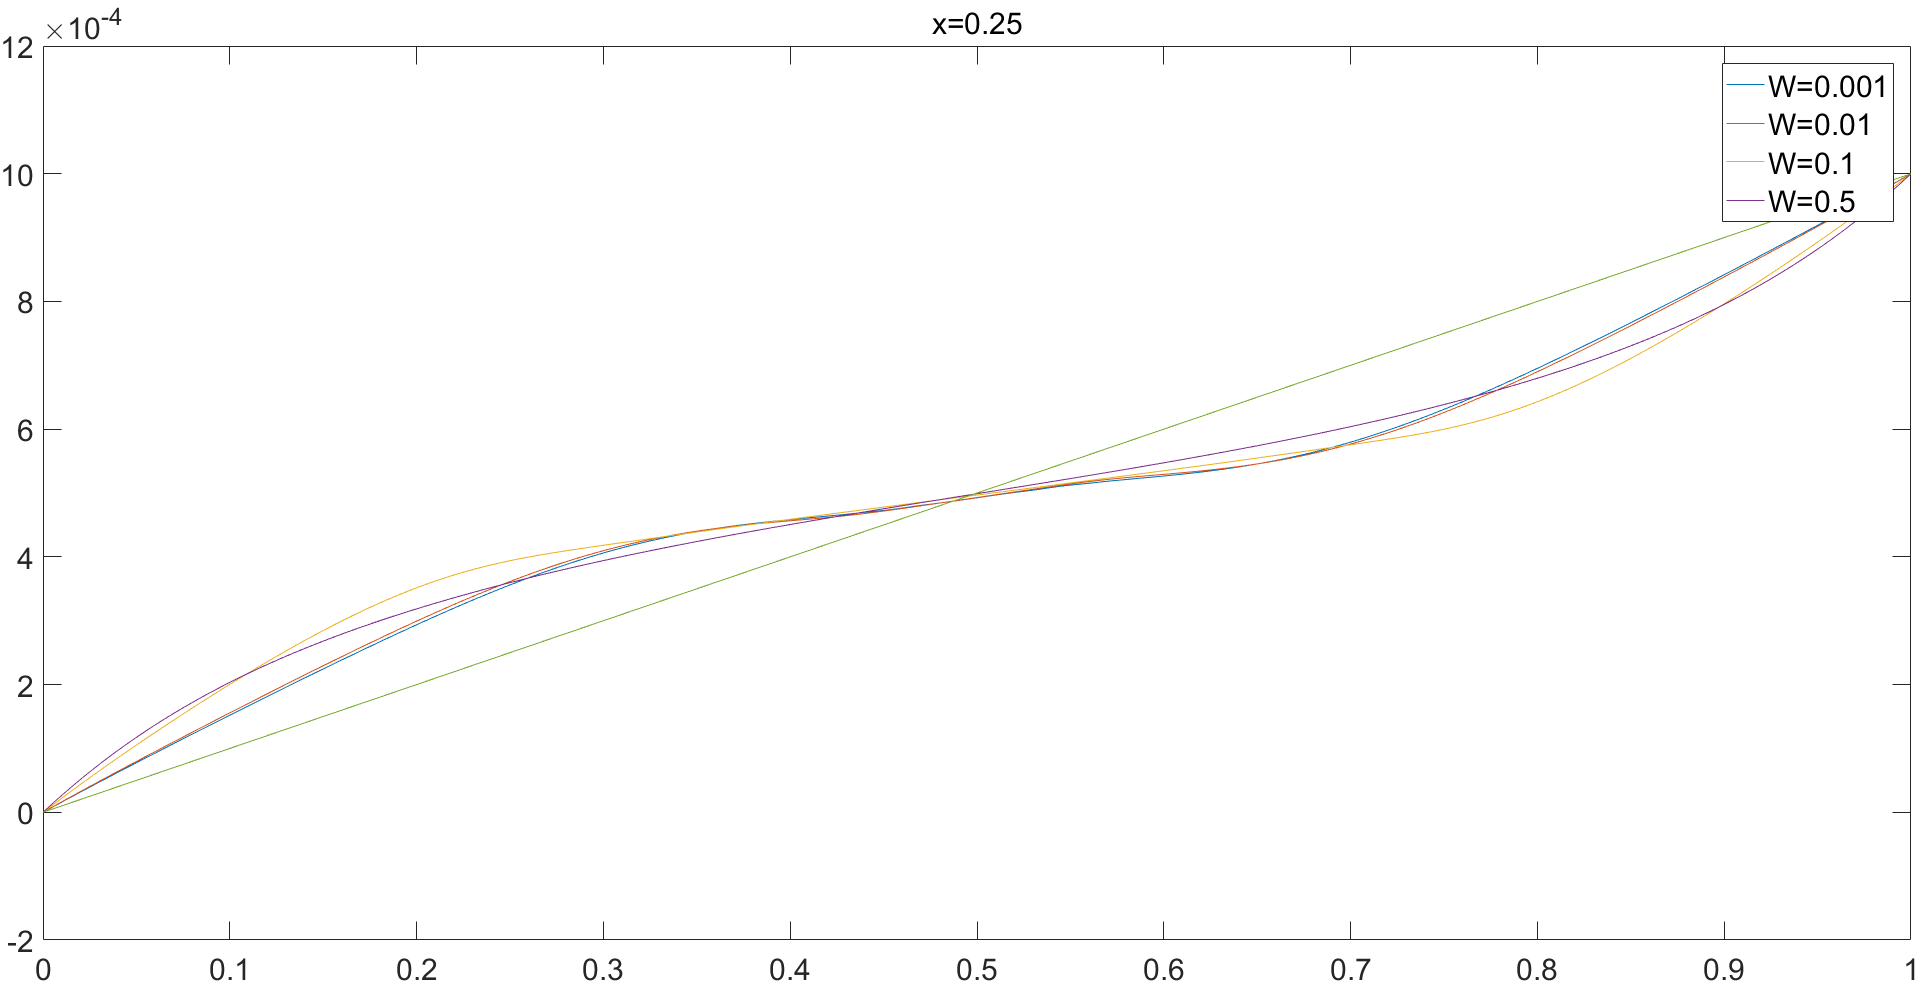
\includegraphics[width=0.8\textwidth]{Circul_P_W/x=0_25.png}}
        \caption{圆形区域下库埃特流速度随着$W$的变化情况:模拟区域为$(x,y)\in [0,1]\times [0,1]$,其中$rate=50,F=0$,标题中$x=0.25$表示曲线为在对应$x$轴位置的3维图形的截线。}
        \label{img12}
    \end{figure}
%pic12
    \begin{figure}[h]
        \centerline{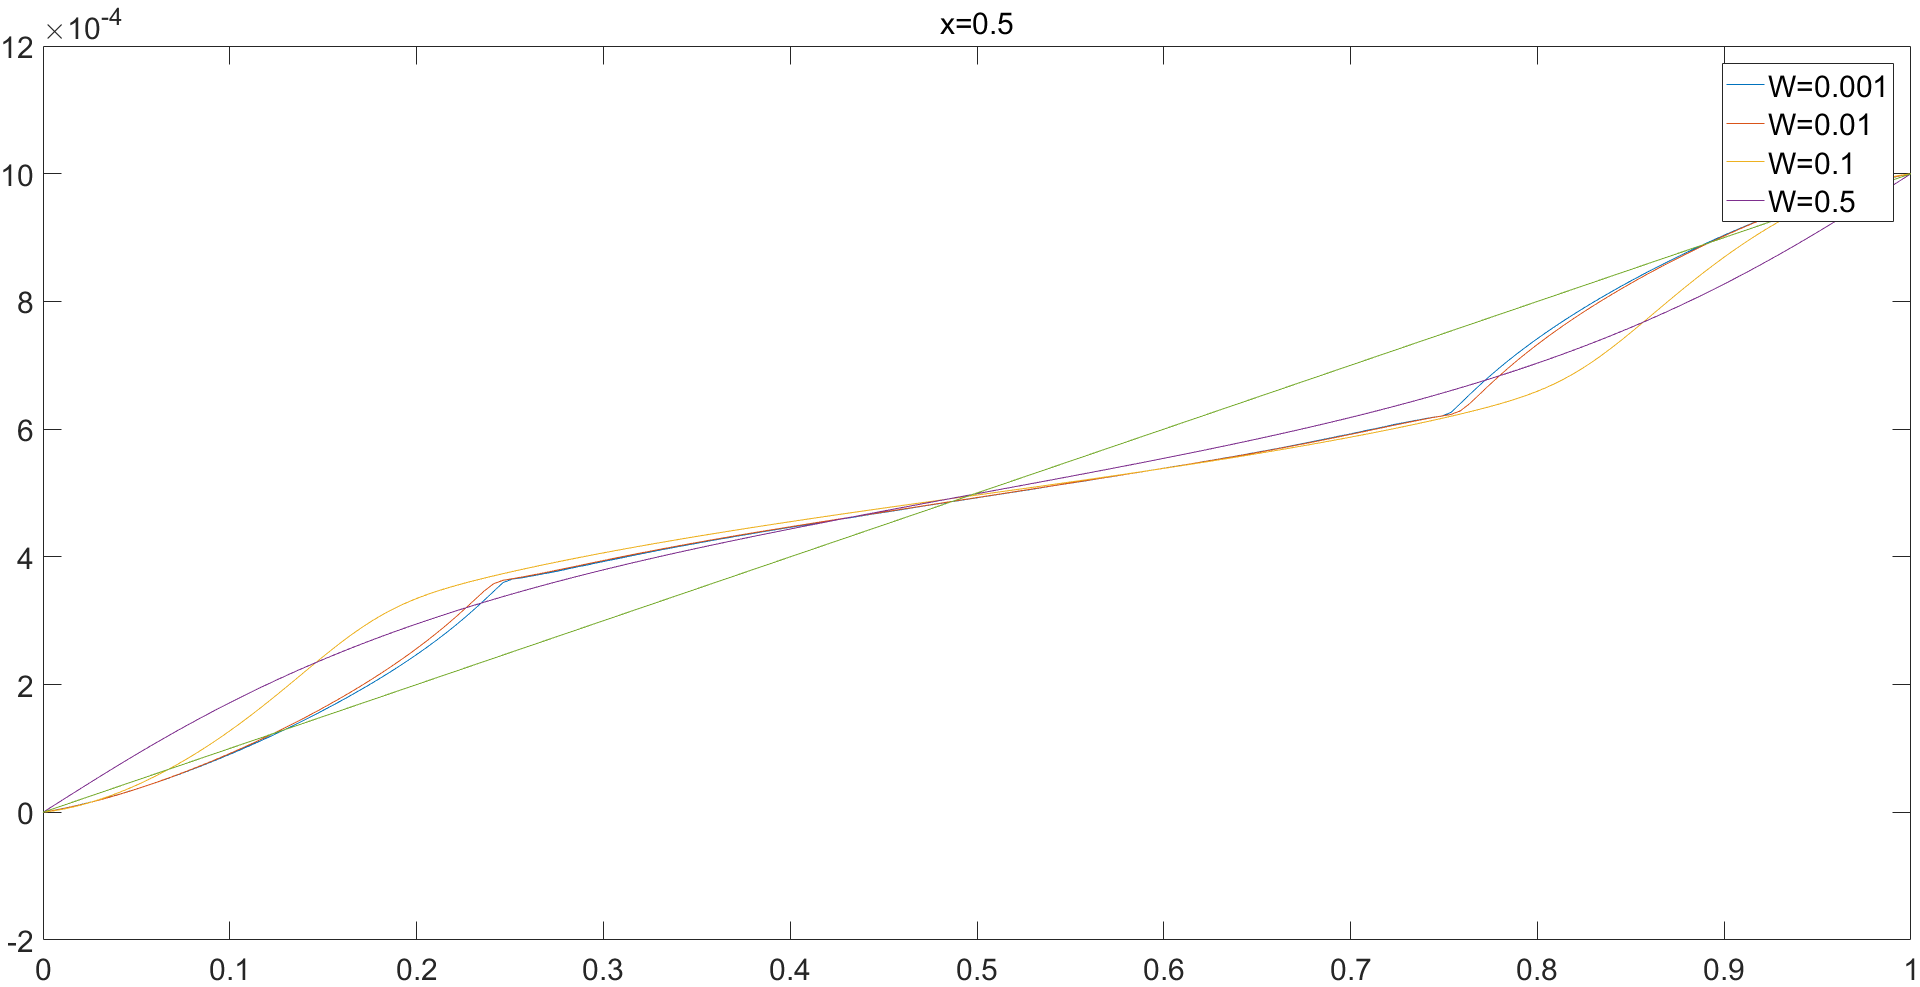
\includegraphics[width=0.8\textwidth]{Circul_P_W/x=0_5.png}}
        \caption{圆形区域下库埃特流速度随着$W$的变化情况:模拟区域为$(x,y)\in [0,1]\times [0,1]$,其中$rate=50,F=0$,标题中$x=0。5$表示曲线为在对应$x$轴位置的3维图形的截线。}
        \label{img13}
    \end{figure}
%pic13
    \begin{figure}[h]
        \centerline{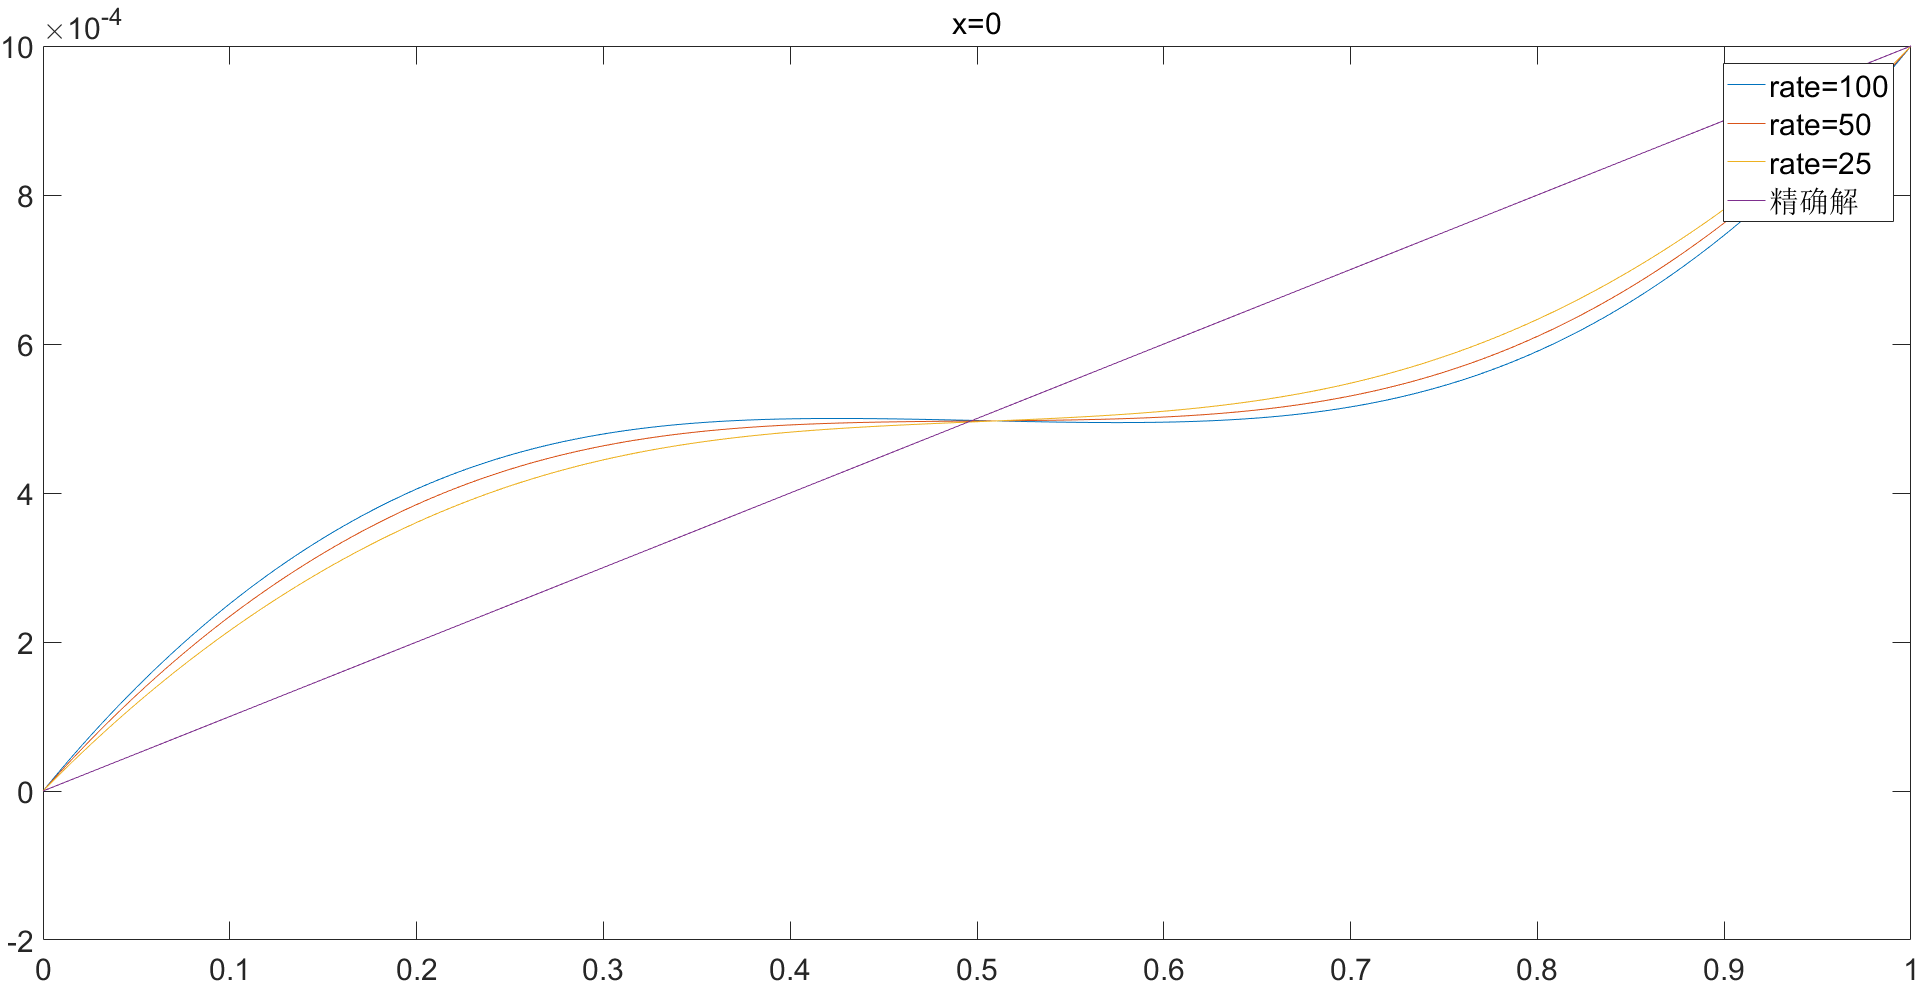
\includegraphics[width=0.8\textwidth]{Circul_P_rate/x=0.png}}
        \caption{圆形区域下库埃特流速度随着$rate$的变化情况:模拟区域为$(x,y)\in [0,1]\times [0,1]$,其中$W=0.1,F=0$,标题中$x=0$表示曲线为在对应$x$轴位置的3维图形的截线。}
        \label{img14}
    \end{figure}
%pic14
    \begin{figure}[h]
        \centerline{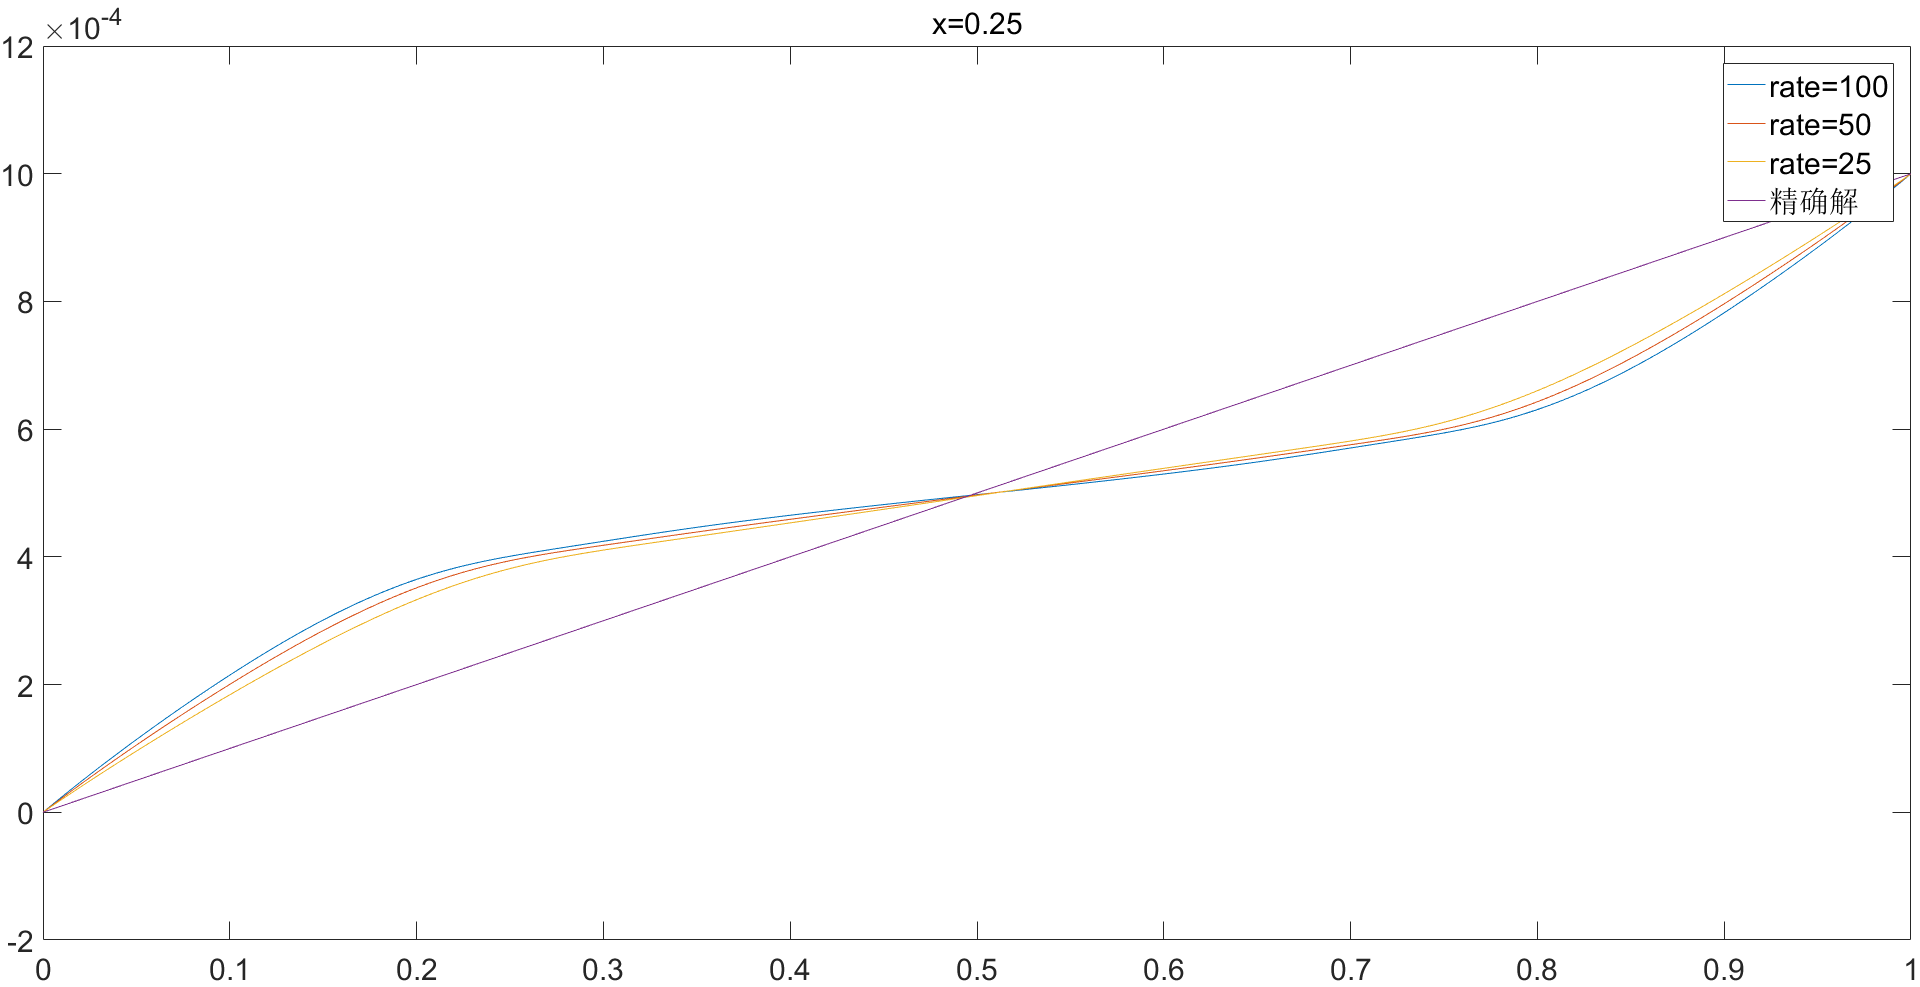
\includegraphics[width=0.8\textwidth]{Circul_P_rate/x=0_25.png}}
        \caption{圆形区域下库埃特流速度随着$rate$的变化情况:模拟区域为$(x,y)\in [0,1]\times [0,1]$,其中$W=0.1,F=0$,标题中$x=0.25$表示曲线为在对应$x$轴位置的3维图形的截线。}
        \label{img15}
    \end{figure}
%pic15
    \begin{figure}[h]
        \centerline{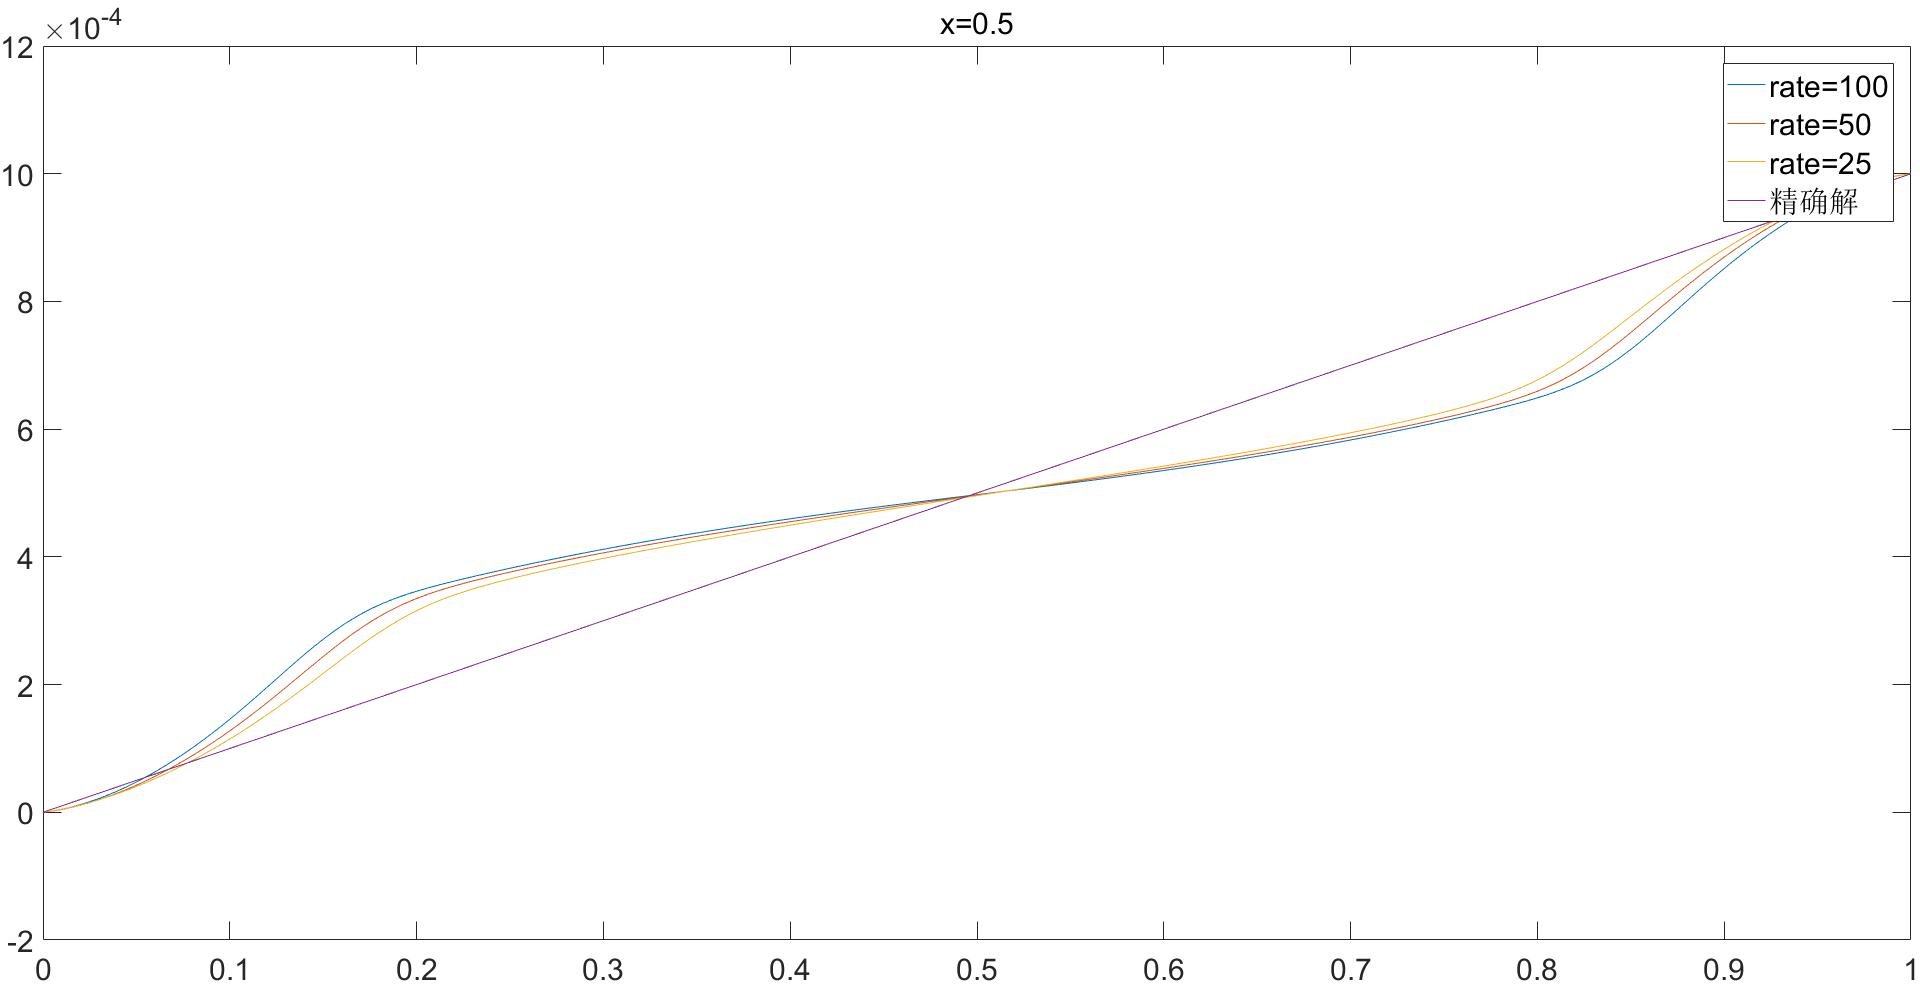
\includegraphics[width=0.8\textwidth]{Circul_P_rate/x=0_5.png}}
        \caption{圆形区域下库埃特流速度随着$rate$的变化情况:模拟区域为$(x,y)\in [0,1]\times [0,1]$,其中$W=0.1,F=0$,标题中$x=0.5$表示曲线为在对应$x$轴位置的3维图形的截线。}
        \label{img16}
    \end{figure}
%pic16
    \begin{figure}[h]
        \centerline{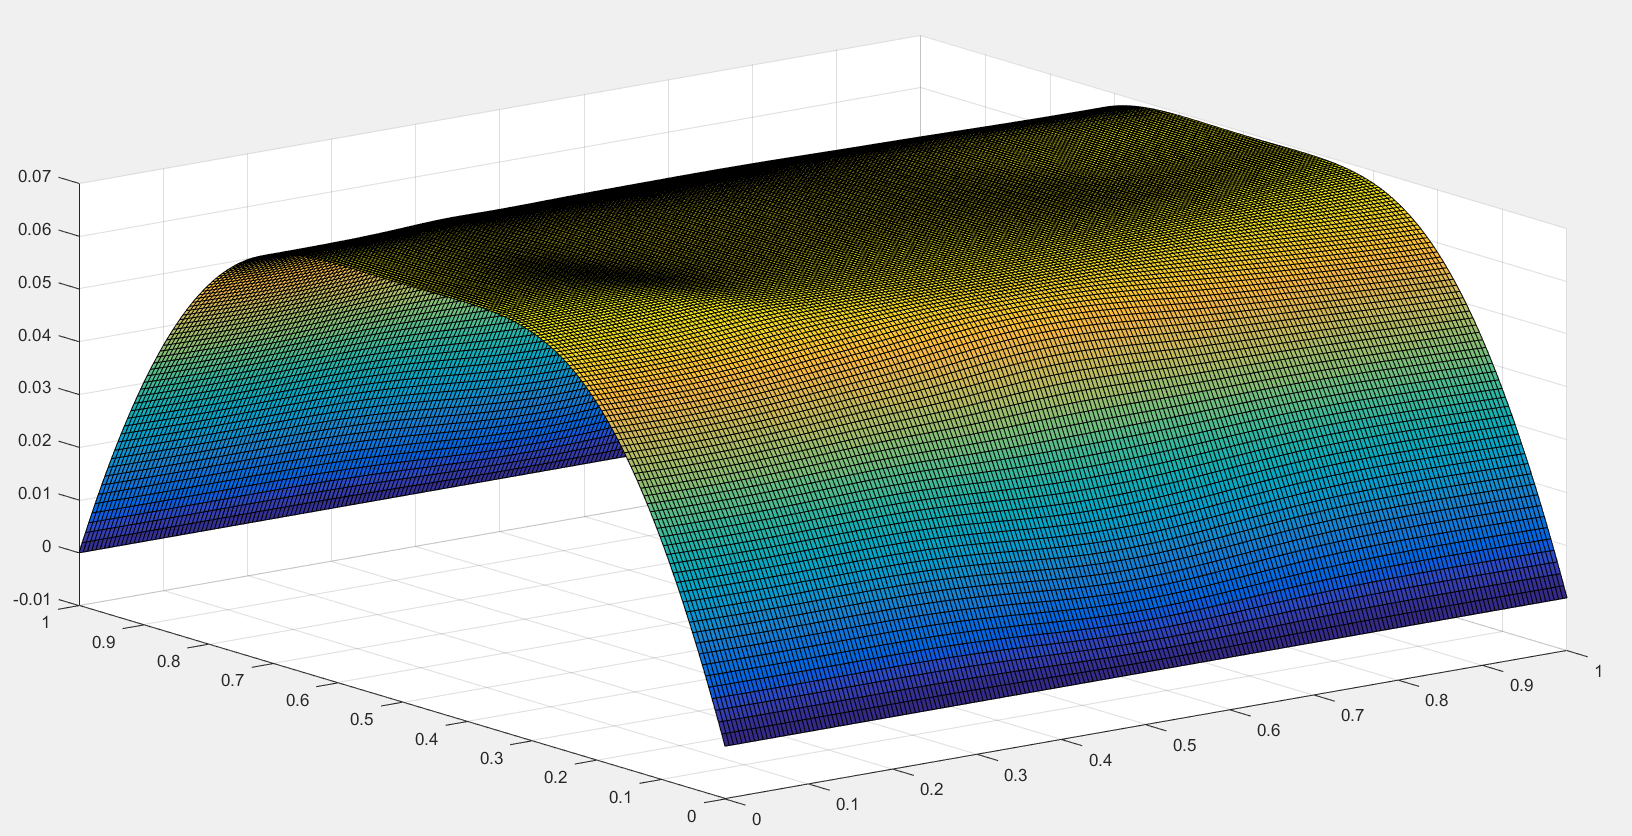
\includegraphics[width=0.8\textwidth]{P_3D.png}}
        \caption{圆形区域下泊肃叶流的2D图像}
        \label{img17}
    \end{figure}
%pic17
    \begin{figure}[h]
        \centerline{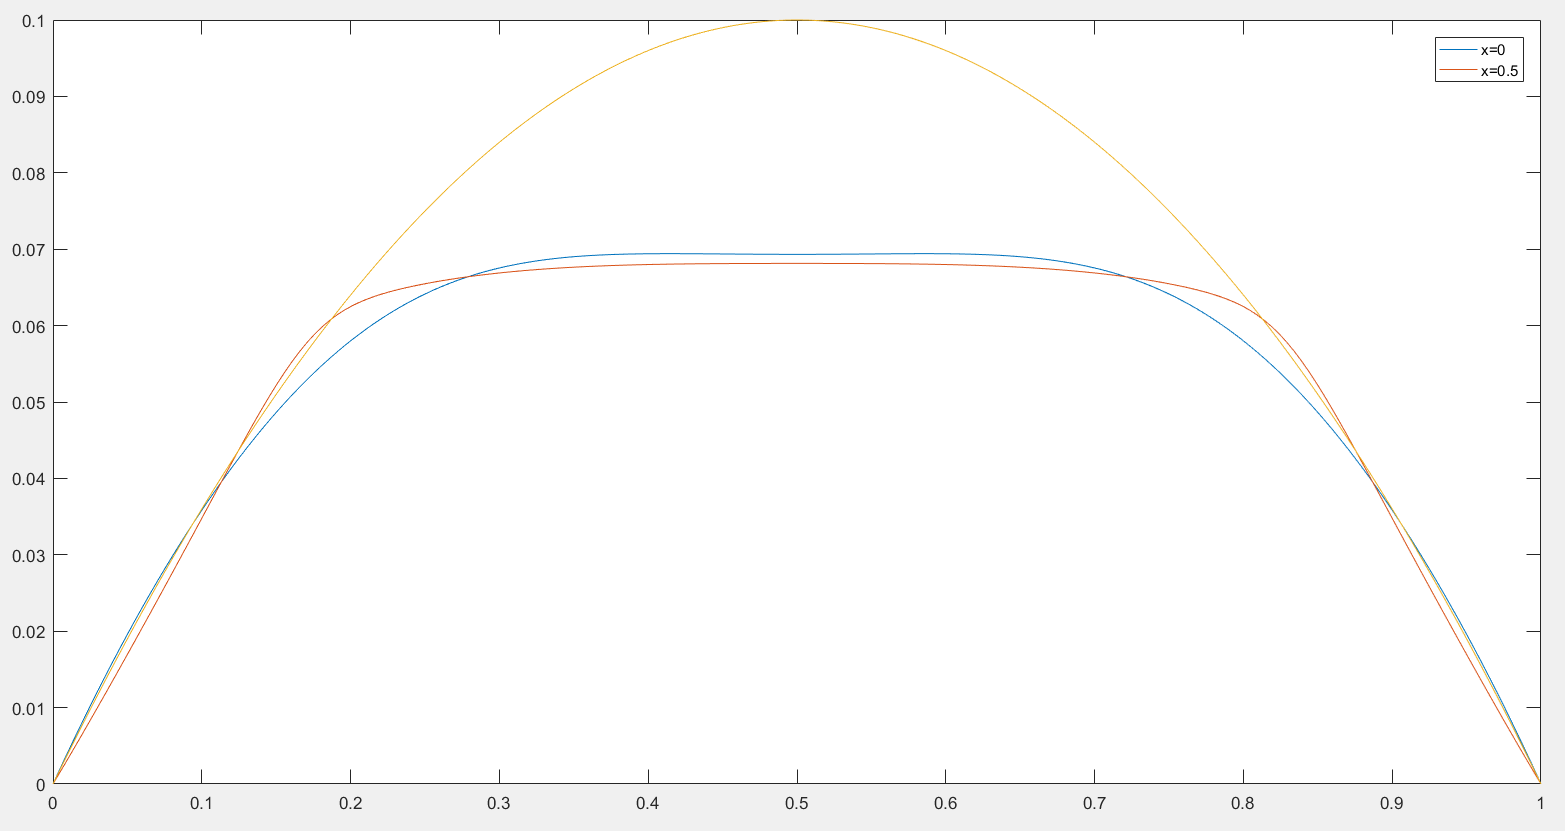
\includegraphics[width=0.8\textwidth]{P_2D.png}}
        \caption{圆形区域下泊肃叶流的2D图像}
        \label{img18}
    \end{figure}
%pic18
    \begin{figure}[h]
        \centerline{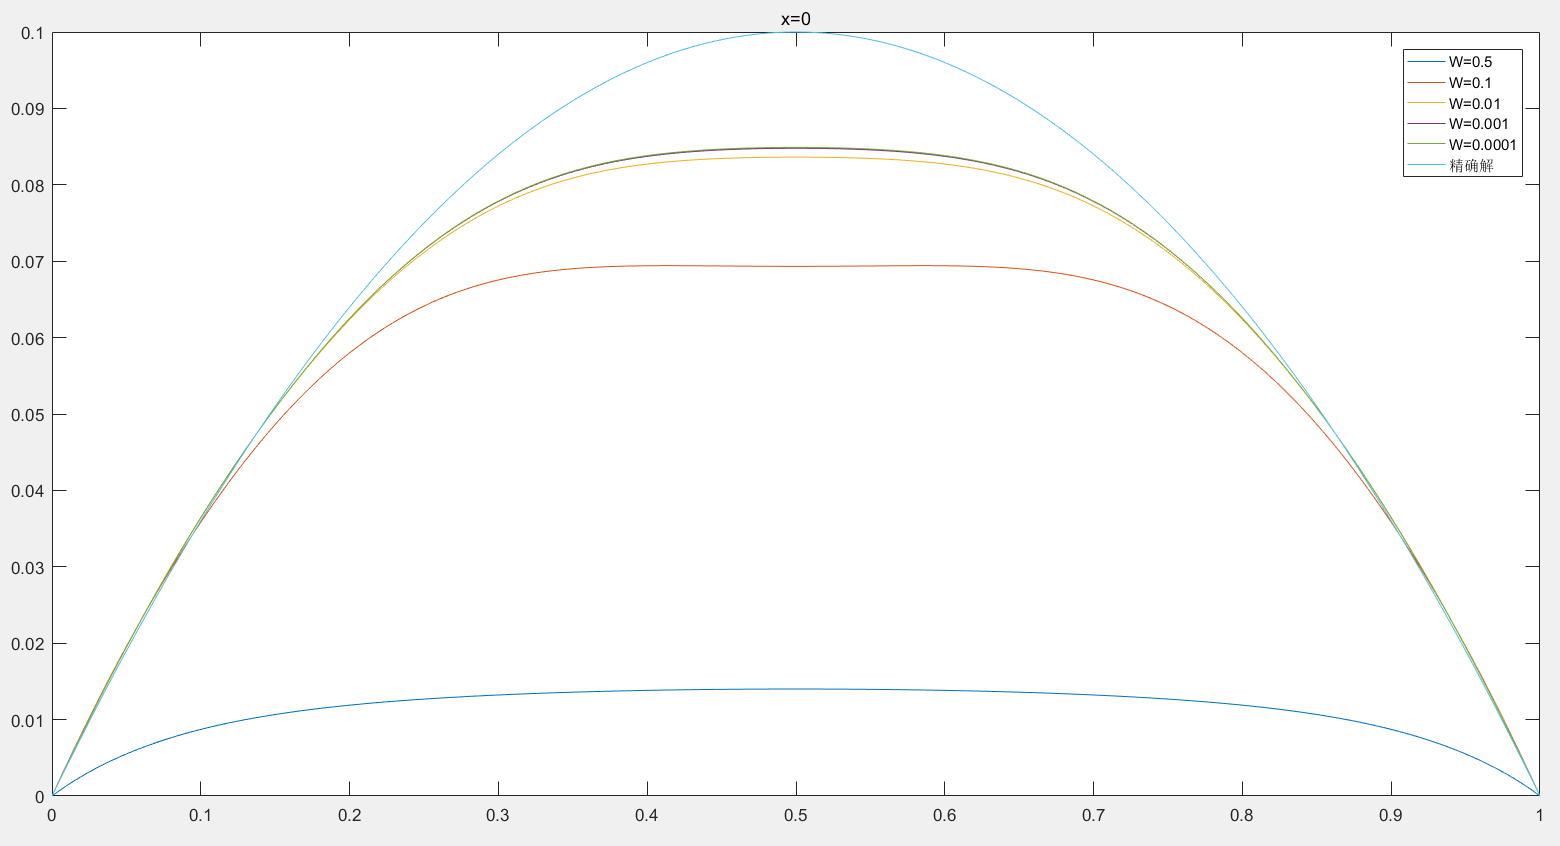
\includegraphics[width=0.8\textwidth]{Circula_F_W_x=0.PNG}}
        \caption{圆形区域下泊肃叶流速度随着$W$的变化情况:模拟区域为$(x,y)\in [0,1]\times [0,1]$,其中$rate=50,Re=500,F=\frac{8\rho u_{peak} \eta_l}{H^2}$,注意力的大小选取和之前不同,标题中$x=0.5$表示曲线为在对应$x$轴位置的3维图形的截线。}
        \label{img19}
    \end{figure}
%pic19
    \begin{figure}[h]
        \centerline{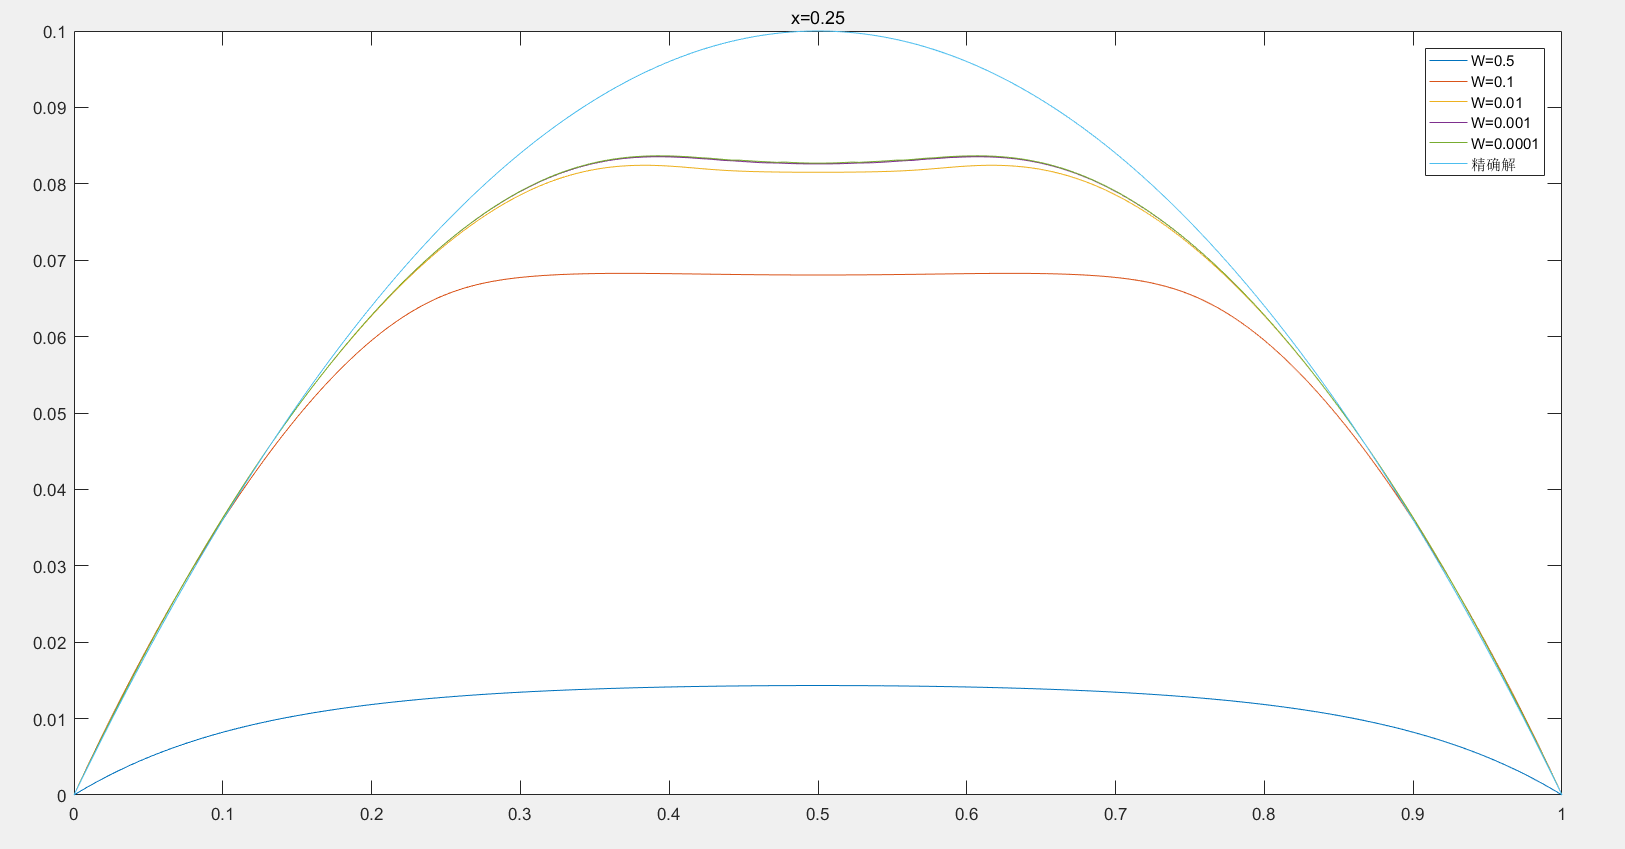
\includegraphics[width=0.8\textwidth]{Circula_F_W_x=0_25.PNG}}
        \caption{圆形区域下泊肃叶流速度随着$W$的变化情况:模拟区域为$(x,y)\in [0,1]\times [0,1]$,其中$rate=50,Re=500,F=\frac{8\rho u_{peak} \eta_l}{H^2}$,注意力的大小选取和之前不同,标题中$x=0.5$表示曲线为在对应$x$轴位置的3维图形的截线。}
        \label{img20}
    \end{figure}
%pic20
    \begin{figure}[h]
        \centerline{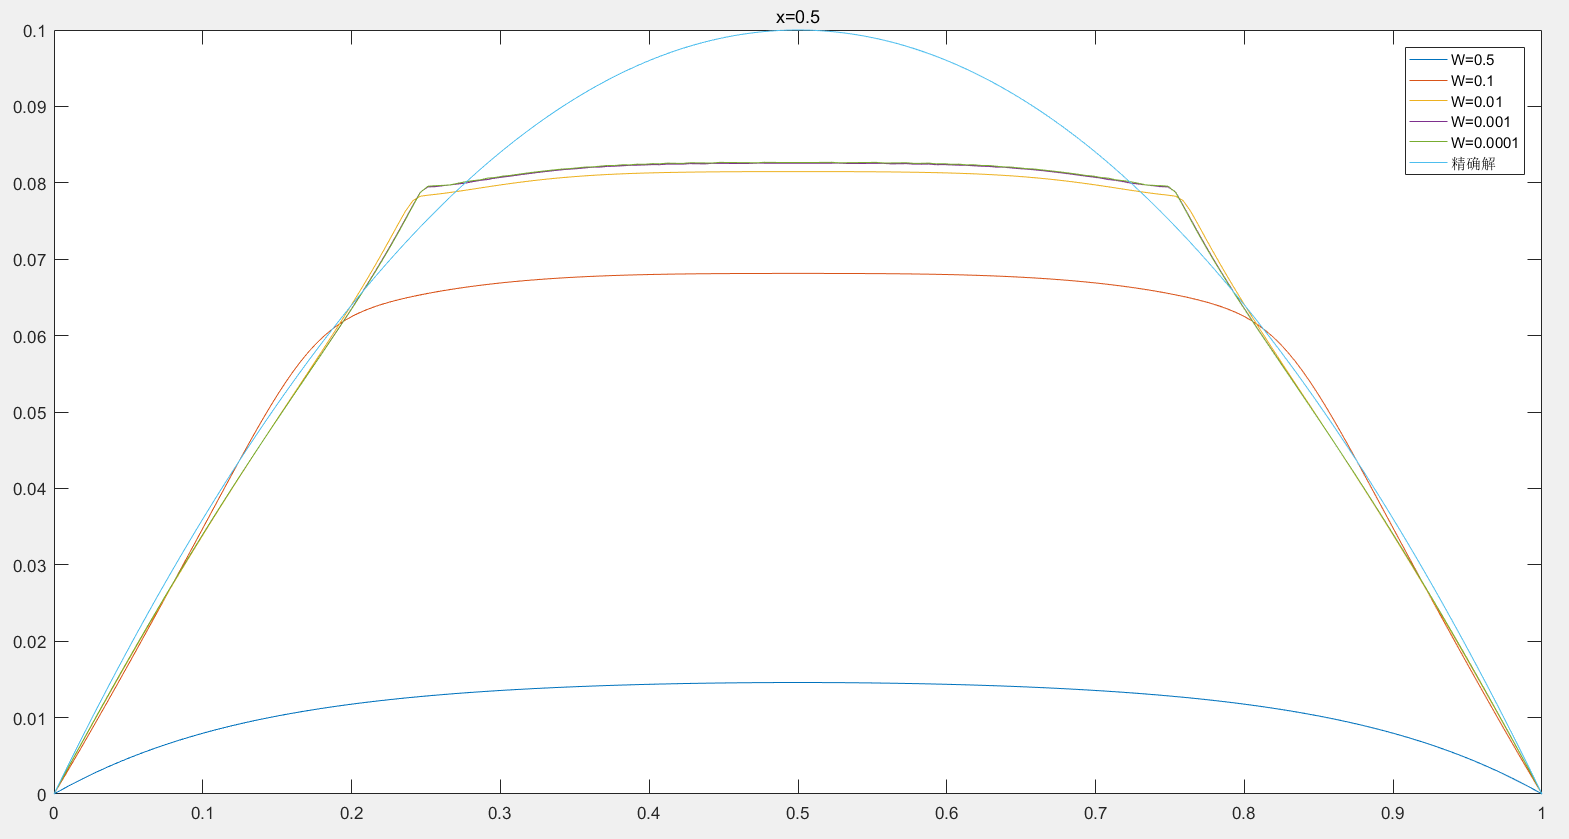
\includegraphics[width=0.8\textwidth]{Circula_F_W_x=0_5.PNG}}
        \caption{圆形区域下泊肃叶流速度随着$W$的变化情况:模拟区域为$(x,y)\in [0,1]\times [0,1]$,其中$rate=50,Re=500,F=\frac{8\rho u_{peak} \eta_l}{H^2}$,注意力的大小选取和之前不同,标题中$x=0.5$表示曲线为在对应$x$轴位置的3维图形的截线。}
        \label{img21}
    \end{figure}
%pic21
    \begin{figure}[h]
        \centerline{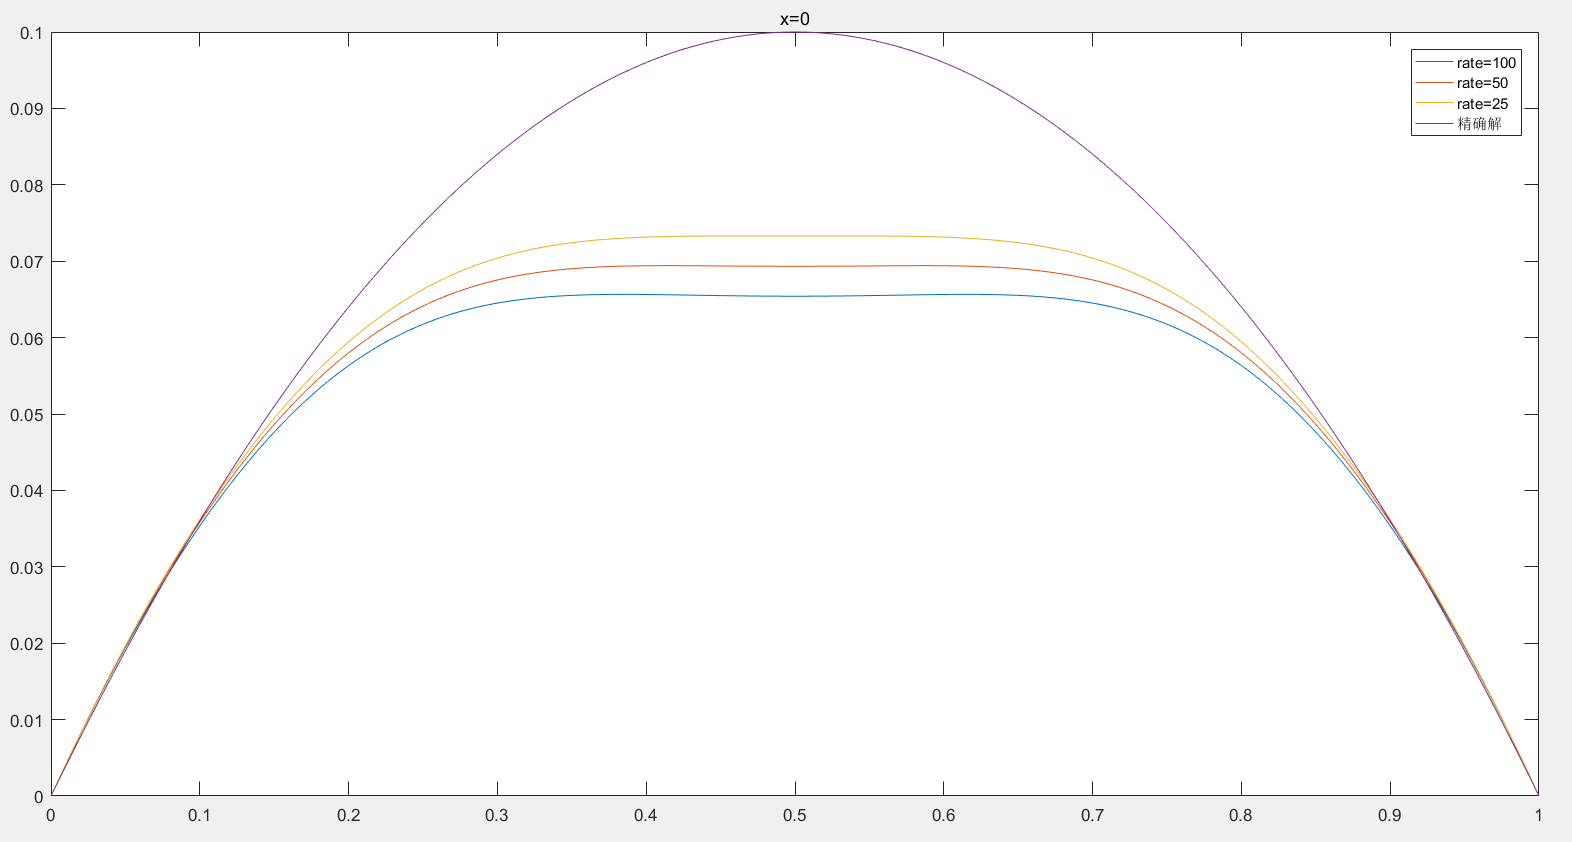
\includegraphics[width=0.8\textwidth]{Circula_F_rate_x=0.PNG}}
        \caption{圆形区域下泊肃叶流速度随着$rate$的变化情况:模拟区域为$(x,y)\in [0,1]\times [0,1]$,其中$W=0.1,Re=500,F=\frac{8\rho u_{peak} \eta_l}{H^2}$,注意力的大小选取和之前不同,标题中$x=0.5$表示曲线为在对应$x$轴位置的3维图形的截线。}
        \label{img22}
    \end{figure}
%pic22
    \begin{figure}[h]
        \centerline{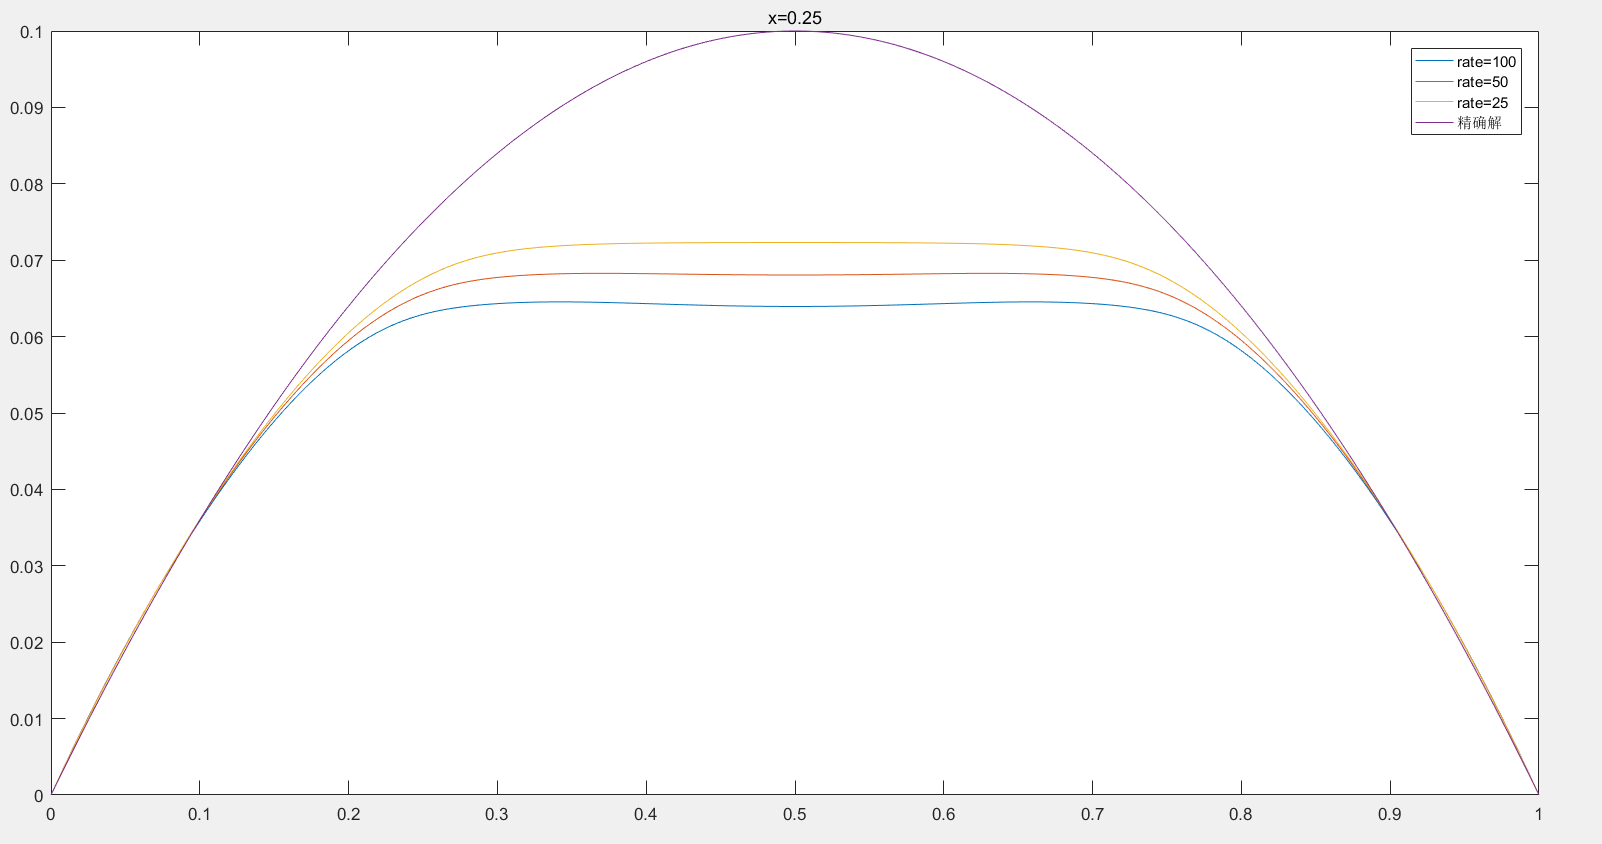
\includegraphics[width=0.8\textwidth]{Circula_F_rate_x=0_25.PNG}}
        \caption{圆形区域下泊肃叶流速度随着$rate$的变化情况:模拟区域为$(x,y)\in [0,1]\times [0,1]$,其中$W=0.1,Re=500,F=\frac{8\rho u_{peak} \eta_l}{H^2}$,注意力的大小选取和之前不同,标题中$x=0.5$表示曲线为在对应$x$轴位置的3维图形的截线。}
        \label{img23}
    \end{figure}
%pic23
    \begin{figure}[h]
        \centerline{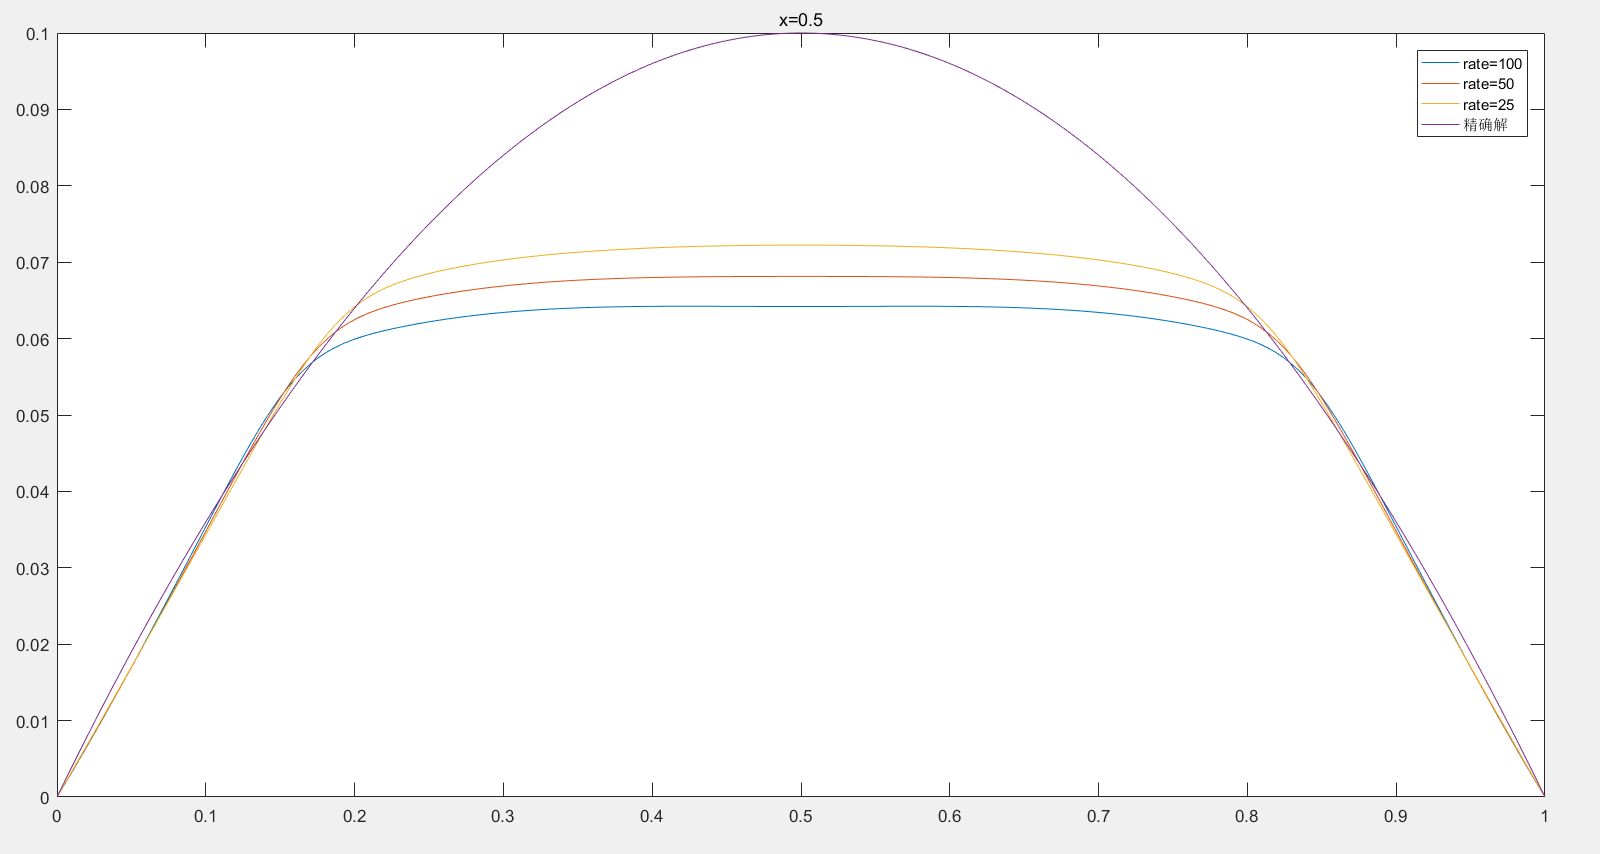
\includegraphics[width=0.8\textwidth]{Circula_F_rate_x=0_5.PNG}}
        \caption{圆形区域下泊肃叶流速度随着$rate$的变化情况:模拟区域为$(x,y)\in [0,1]\times [0,1]$,其中$W=0.1,Re=500,F=\frac{8\rho u_{peak} \eta_l}{H^2}$,注意力的大小选取和之前不同,标题中$x=0.5$表示曲线为在对应$x$轴位置的3维图形的截线。}
        \label{img24}
    \end{figure}
%pic24
    %%\begin{figure}[h]
        %%\centerline{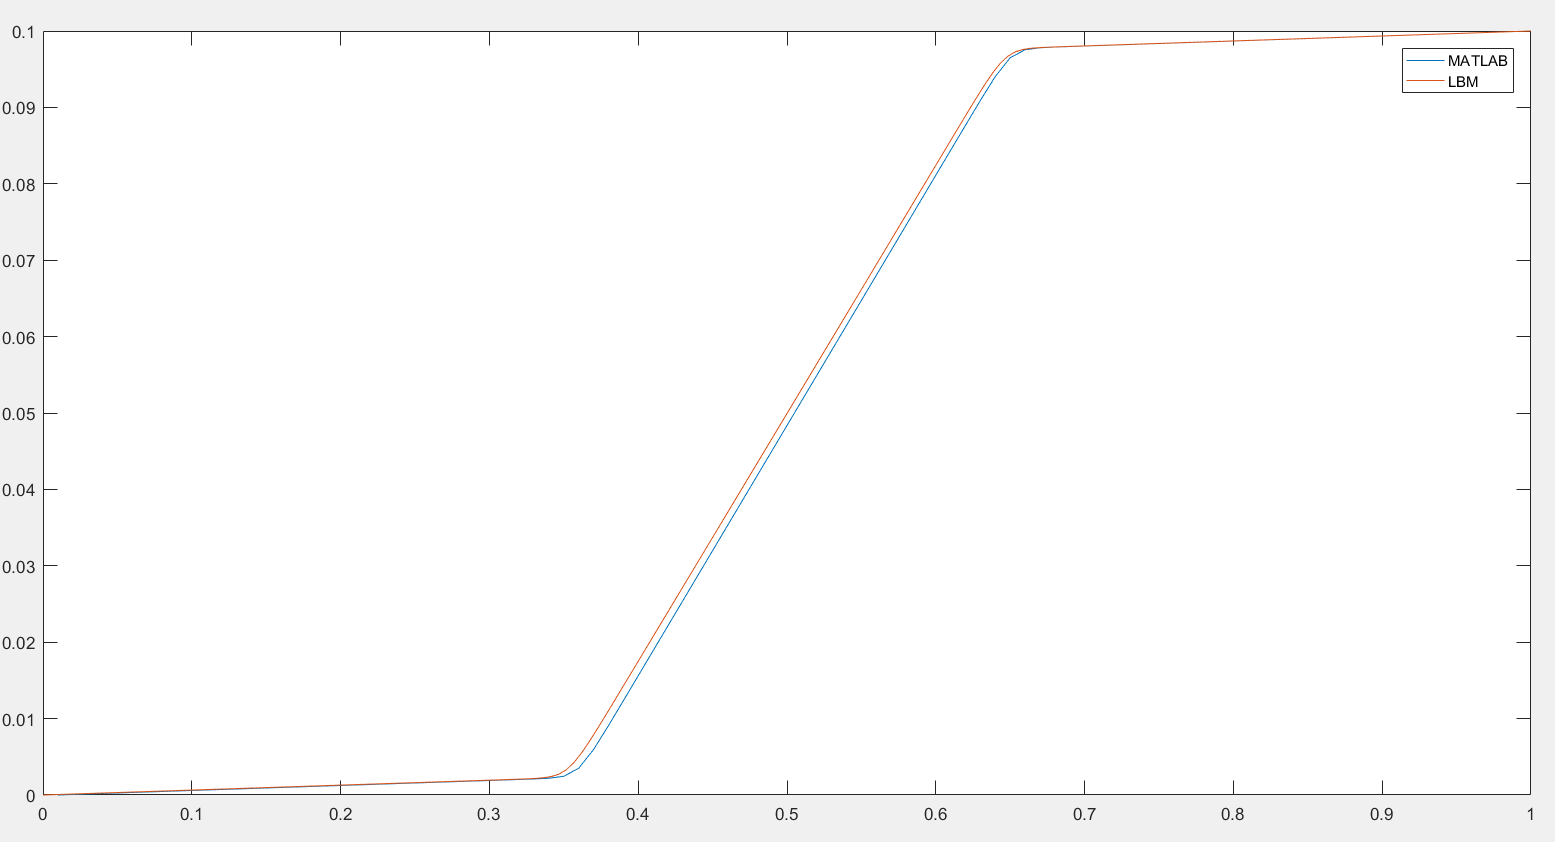
\includegraphics[width=0.8\textwidth]{C_0_01.PNG}}
        %%\caption{平行区域库埃特流下MATLAB与LBM模拟结果的比较:模拟进行在库埃特流下,参数为$W=0.01,rate=50,Re=500,F=0$。}
        %%\label{img25}
    %%\end{figure}
%pic25
    %%\begin{figure}[h]
        %%\centerline{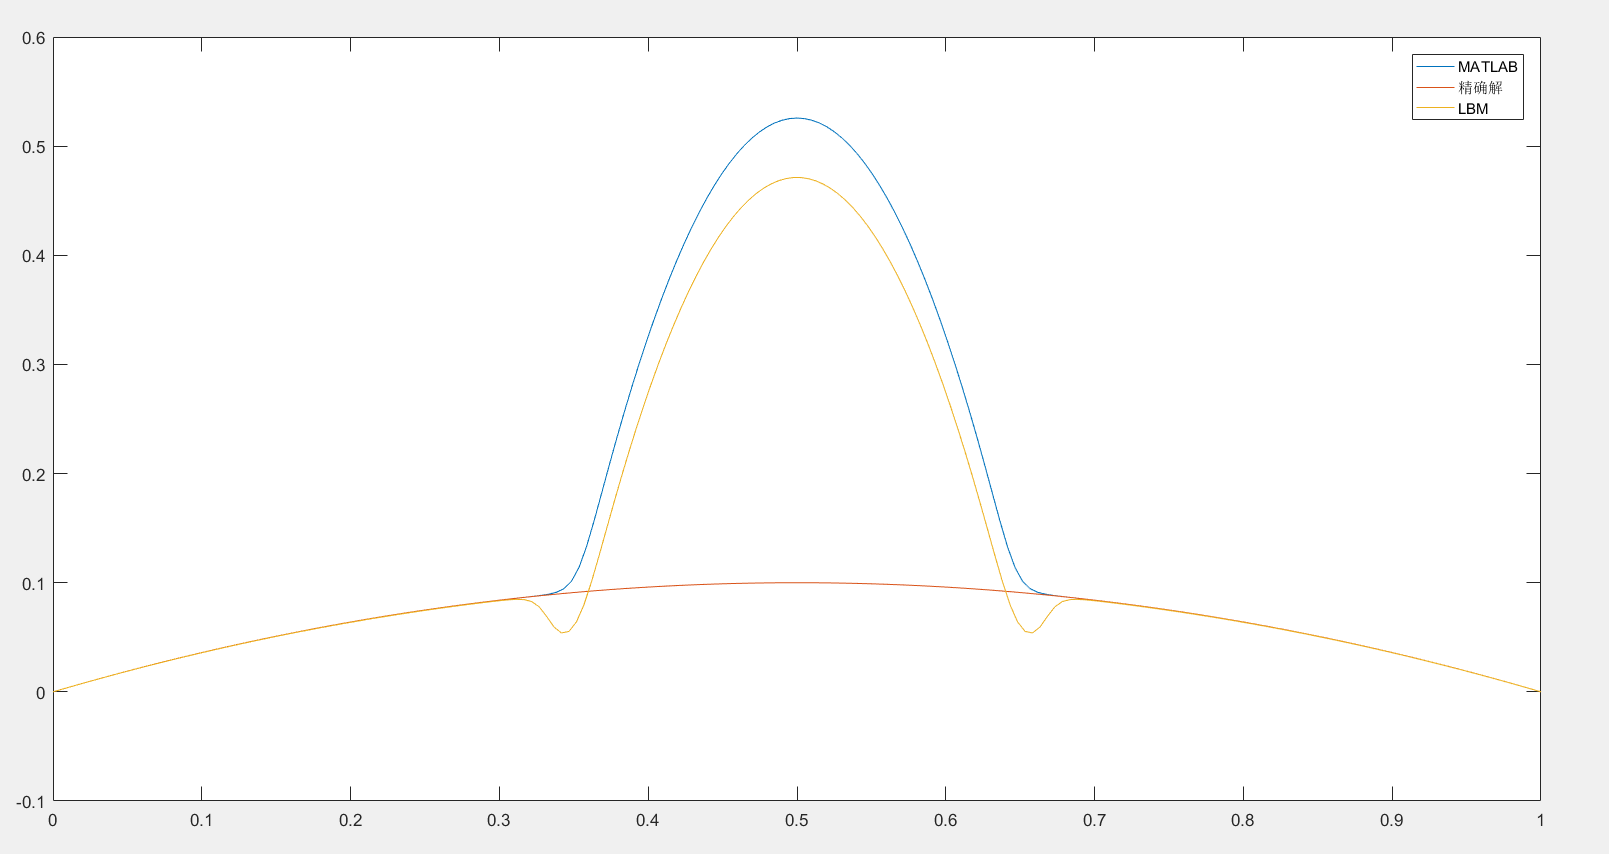
\includegraphics[width=0.8\textwidth]{F_0_01.PNG}}
        %%\caption{平行区域泊肃叶流下MATLAB与LBM模拟结果的比较:模拟进行在泊肃叶下,参数为$W=0.01,rate=50,Re=500,F=\frac{8\rho u_{peak} \eta_l}{H^2}$。}
        %%\label{img26}
    %%\end{figure}
\end{document}